\documentclass[11pt,a4paper]{amsart}
\usepackage{geometry, empheq}
\usepackage[english]{babel}
%\pagestyle{myheadings}
%\textheight25.3cm
%\oddsidemargin 1cm
%\evensidemargin 1cm
\usepackage{amsmath}
%\usepackage{showkeys}
\usepackage{amssymb}
\usepackage{amsthm}
\usepackage{xcolor,graphicx}
\usepackage{color}
\usepackage{varioref}
\usepackage{nicefrac}
\usepackage{caption}
\usepackage{subcaption}
\usepackage{float}
\usepackage[normalem]{ulem}
\usepackage{multirow}
\usepackage{enumerate}
\usepackage[colorinlistoftodos]{todonotes}
\usepackage{amsfonts}
\usepackage{booktabs}
\usepackage{siunitx}
%\usepackage{hyperref}
%\usepackage{tikz}
%\usepackage{pgfplots} 
%\usepackage{pgfgantt}
%\usepackage{pdflscape}
%\usepgfplotslibrary{external} 
%\tikzexternalize
%\pgfplotsset{compat=newest} 
%\pgfplotsset{plot coordinates/math parser=false}
\usepackage{algorithm}
\usepackage{algorithmic}
\usepackage{comment}
\usepackage{caption}
\captionsetup{skip=5pt}
%\usepackage{url}

%\selectcolormodel{gray}
\def\b#1{{\mbox{\boldmath $#1$}}}
\def\lewz#1{\leqno(#1)}
%\usepackage{booktabs}
\newcommand{\ak}{\hspace{20pt}}
\newcommand{\bak}{\parindent=0pt}
\newcommand{\sm}{\smallskip}
%\newcommand{\smallskip}{\medskip}
\newcommand{\bs}{\bigskip}
\newcommand{\arrow}{\rightarrow}
\newcommand{\ds}{\displaystyle}
\newcommand{\kr}{\hspace{-0.2cm}{\bf.~}}
\newcommand{\kw}{\rule{2mm}{2mm}}
\newcommand{\ged}{\hfill\kw}
\newcommand{\pf}{\b{Proof.} \ }
\newcommand{\ssn}{({\bf SSN}) }
\renewcommand{\div}{\text{div\,}}
\newtheorem{example}{\textbf{Example}}
%\newcommand{\norm}[1]{{\|  #1\|}}
\renewcommand{\l}{\left}
\renewcommand{\r}{\right}
\newcommand{\om}{\Omega}
\newcommand{\ga}{\Gamma}
\newcommand{\fsparse}{\Upsilon}
\newcommand{\reals}{\mathbb{R}}
\newcommand{\sign}{\mathrm{sign}}
\newcommand{\warrow}{\rightharpoonup}
\def\thesection{\arabic{section}}
\def\thesubsection{\arabic{section}.\arabic{subsection}}
\def\thefigure{\arabic{figure}\normalfont}
\def\thetable{\arabic{table}\normalfont}
\setcounter{table}{0}
\newcommand{\nota}[1]{ \colorbox{red}{\textcolor{white}{\tiny{#1}}}}
\DeclareMathOperator{\argmin}{argmin}
%\newenvironment{proof}[1][Proof]{\b{Proof.}{\hfill\kw}}
\renewenvironment{proof}{{Proof.}}{\hfill\kw}

%\font\nowa = eufm5 scaled \magstep 3
\font\tenpoint=cmr10
\font\ninepoint=cmr9
\newcounter{theassumption}
\setcounter{theassumption}{0}
\newtheorem{assumption}[theassumption]{{Assumption}}
\newtheorem{proposition}{{Proposition}}
\newtheorem{definition}{{Definition}}
\newtheorem{lemma}{{Lemma}}
\newtheorem{remark}{{Remark}}
\newtheorem{corollary}{{Corollary}}
\newtheorem{theorem}{{Theorem}}
\newcommand{\cor}{\color{red}}
\newcommand{\norm}[1]{\lVert #1 \rVert}
\newcommand{\subtag}[1]{\tag{\theparentequation#1}}
%\addbibresource{biblio.bib}

\begin{document}
	\title[Nonconvex optimal control problems]{ Mixed--constrained elliptic optimal control problems with $L^q$--quasinorm penalization}
	%\title{Numerical solution of nonconvex PDE--constrained optimization problems via DC programing}
	
	\author{Pedro Merino$^\ddag$ and Diego Vargas$^\ddag$}
	%\address{}
	\address{$^\ddag$Research Center of Mathematical Modeling (MODEMAT) and Department of Mathematics, Escuela Polit\'ecnica Nacional, Quito, Ecuador}
	\keywords{}
	\subjclass[2010]{90C26, 90C46, 49J20, 49K20}
	\thanks{$^*$This research has been supported by Research Project PIMI-17-01 funded by Escuela Polit\'ecnica Nacional, Quito--Ecuador.}
	
	\smallskip
\begin{abstract}
In this paper we study a nonconvex optimal control problem with sparsity induced by a $L^q$-quasi norm penalty ($0<q<1$), and when mixed point wise constraints are imposed. We discuss the numerical solution of such problems, considering a method that combines the DC-Method (Difference-of-convex functions algorithm) together with the semi smooth Newton method, and which was derived from the optimality conditions of a regularized problem using the DC--programming approach.
\end{abstract}
	
\maketitle 




\section{Introduction}

In the theory of optimal control problems governed by partial differential equations, the use of penalties in the cost function which induces sparsity on the optimal control, and the presence of mixed--constrained restrictions over the control and state of the problem, are widely studied and used for many theoretical and practical problems, but in a separated way. However, as far as we know, there are few literature about problems which combines these two paradigms in only one optimal control problem, despite the relevance that each individual paradigm could represent. For example, problems with penalties using $L^q$ quasi norms, with $q\in [0,1)$ are well known for inducing sparcity over the optimal control solution, see for example \cite{ito-kunish, merino}, likewise the $L^1$ penalization in the cost function studied, for example, by Stadler \cite{stadler}; therefore, such characteristic over the optimal control could be used for placement of technological equipment, inverse problems in biomedical or seismic imaging, certain energy efficiency models (see \cite{vogel}), image restoration (see \cite{hinttv}), compressed sensing (see \cite{donoho}) and optimal control problems (see \cite{casas}). However, the main difficult in the treatment of the quasi-norm penalized problems is the obvious lack of convexity in the cost function, which implies that the use of standard techniques of the Convex Analysis cannot be applied for the derivation of a solution and an optimally system for it.\\ 

On the other hand, optimal control problems which present restrictions over the control and state are studied by several authors, see for example \cite{casas, casas-kunisch, casas-delosreyes}, etc. Those problems are important in practical uses, for example, problems involved with heat phenomena, elasticity theory, flux theory, finances and over all problems which demands that the state must be in specific set \cite{hintkun}. However, when we impose point-wise state constrains in some optimal control problems with convex cost function, it was shown that the Lagrange multipliers that appears in the optimal systems have poor regularity, see for example \cite{casas, casas-delosreyes}. This result introduces a new challenge in the study of this kind of problems, because the lack of sufficient regularity for the Lagrange multipliers arisen from the optimal system above implies that their numerical treatment could be difficult. Even the active-set strategies proposed by Bergounioux, Ito and Kunisch \cite{bik}, Bergounioux and Kunisch \cite{bk}, or Kunisch and Rosch \cite{kr}, cannot be applied for its numerical treatment. However, in \cite{meyer1} it is introduced a technique for witch we get a sub problem with $L^2$ Lagrange multipliers. This technique consists in defining an artificial control which involves the originals states and control of the problem and reformulate the original optimal control problem with the new artificial control. This process is called a \textit{Lavrentiev regularization} for the problem, and the main idea of this is to interchange the point-wise constrains from the original state to the new defined control.\\

 For the numerical analysis of problems with non convex penalties, it is frequently used a well-known technique called Newton's semi-smooth method, which was first introduced by Mifflin in \cite{mifflin} for the study of problems defined on finite-dimensional spaces, and then it was extended to problems on infinite dimensional spaces by Qi and Sun \cite{qi}, \cite{qisun}. The importance of the semi-smooth method lies in the fact that it can be applied to solve equations of the form $F(x)=0$, being $F$ some function or functional on a Banach space, imitating Newton's classical algorithm for solving equations; but the main difference between these two methods is that $F$ does not have necessary sufficient regularity, such as a $C^1$ regularity on its domain. For this reason, we use the theory of Newton semi smooth methods developed in \cite{ulbrich} in order to determinate the numerical solution of our problem particularized to a certain PDE equations. \\

In this work we study a certain type of optimal control problem which presents a $L^q$ quasi norm penalization, $q\in ]0,1[$, and mixed control and state point-wise constraints; being these restrictions inspired in a Lavrentiev-type mix of control and state point-wise restrictions. Specifically, we demonstrate that our problem has a solution which can be used for the study of another control problem with a $L^q$ penalization and pure state point-wise state constraints. Then, we derive an optimal system for the penalized problem with pure state point-wise constraints, using the theory of Difference of Convex functions. Finally we develop a numerical algorithm for solving it, using the semi smooth Newton scheme and then we present our numerical results.\\

This paper is organized as follows: in the Section 2 we introduce our problem and some useful notations for this work. In Section 3 we introduce a regularization of the $L^q$ penalty present in our control problem, using the so called Convex regularization or $\Gamma-$regularization (see \cite{eck}), for deducing optimal systems that will be used after. In section 4 we present a $L^q$ penalized control problem with only point-wise state constrains, which can be seen as a particular case of the problem present in Section 2. In this chapter also we study the existence of solutions for it, using the results developed in Section 3. In Section 5 we deduce optimally conditions for the $L^q$ penalized problem with only point-wise state constrains, using the DC theory (Difference of Convex functions theory, see \cite{merino, dihn}). In Section 6 we use the semi smooth Newton method for the numerical analysis of our results, using the optimal system deduced in Section 5. We finalize this paper with our conclusions.

 \section{Preliminaries and notations}
Let $\om \in \reals^{n}$ be a bounded domain with $n=2, 3$ and with a Lipschitz boundary $\Gamma$. Let  $a_{ij}$ be Lipschitz continuous functions for all $i,j\in \{1,\cdots,n\}$  such that there exist a positive constant $\alpha>0$, such that
\begin{equation}\label{pdecondition}
    \sum_{i,j=1}^{n}a_{ij}(x)\xi_{i}\xi_{j} \ge \alpha\norm{\xi}^2, \quad \forall  (x,\xi)\in \om\times\reals^n
\end{equation}
Let $A$ be a second-order differential operator defined by
\[
    Ay=-\sum_{i,j=1}^{n}\dfrac{\partial}{\partial x_j}\l(a_{ij} \dfrac{\partial}{\partial x_i}y\r)+a_0y,
\]
with {\color{red}$a_0\in L^{\infty}(\om)$, $a_0(x)\ge 0$ a.e. $x\in \om$. [dónde se usa esto?]}

For given real positive constants  $\alpha$, $\beta$, $\lambda$ and $q\in (0,1)$ and $\lambda>0$, we are interested in the mixed control-state constrained optimal control problem:
\begin{equation}\label{plambda}\tag{$P_{\lambda}$}
    \begin{cases}
    \displaystyle\min_{(y,u)\in H^1(\om)\times L^2(\om)}\; \frac{1}{2}\norm{y-y_d}^2_{L^2(\om)}+\frac{\alpha}{2}\norm{u}^2_{L^2(\om)}+\beta \int_{\om} |u|^{q}\; dx\\
    \mbox{subject to:}\\
    Ay(x)=u(x), \phantom{aaaaa} \mbox{in } \om,\\
    \partial_{\Vec{n}}y(x)=0, \phantom{aaaaaaaaaaaaa} \mbox{over } \Gamma,\\    
    y_a\le y(x)+\lambda u(x)\le y_b,\phantom{a} \mbox{almost all }x\in \Omega
    \end{cases}
\end{equation}

with $y_a, y_b$ real constants. 

\begin{remark}
    Mixed constraints are also motivated by Lavrentiev type regularization in the presence of point-wise state constrains, see \cite{meyer1}. 
    The main reason behind this consideration can be explained as follows: first of all, if we define the problem $P_0$ as same as the problem $P_{\lambda}$ except for the point-wise restriction that we replace by $$y_a\le y(x)\le y_b,\quad \text{for almost all } x\in \Omega.$$
    
     Thus, $(P_{0})$ is a non convex problem with point-wise state constraints. Such problems are practical and theoretical interesting. However, since the cost function is not convex, the existence of a solution for $P_0$ cannot be followed by the usual direct methods. They require special techniques of regularization for the non convex term present in this cost function. Nevertheless, the relation between the solutions of the regularized problem $P_0$ and the non regularized $P_0$ are not enough clear. We avoid this difficult following a different way for demonstrating solutions for the non regularized $P_0$. In the first place, we consider the family of regularized problems $P_{\lambda}$ with $\lambda>0$, using the so called  \textit{Convex regularization} or $\Gamma-$\textit{regularization} of the problem (see \cite{eck}). This method consists in the substitution of the original non convex cost function of \eqref{P} for a convex version of it, constructed from the convex envelope of the one dimensional non convex penalty presented in \eqref{P}. The virtue of using such problems is that the optimal systems arisen from each one, produces a sequence of multipliers with converges as $\lambda\to 0$ to certain functions which will be used for demonstrating that the non regularized problem $P_0$ has at least one solution.
\end{remark}
 

We introduce some useful notations: first of all, the classic Lebesgue and Sobolev spaces will be denoted with the usual $L^p(\Omega)$ and $W^{k,p}(\Omega)$ notations. Here $H^1(\Omega)=W^{1,2}(\Omega)$. Of course we will use the standar norm notations $\norm{\cdot}_{L^p(\Omega)}$ and $\norm{\cdot}_{W^{k,p}(\Omega)}$, too. The classical notation for convex sub differentials of a convex function $f$ will be $\partial f$. Let $E$ a Banach space and $V\subset E$; the indicator function over $V$ is defined as
\[
\mathbf{I}_{V}(x)=\begin{cases}
    0,& x\in V\\
    +\infty,&x\notin V,
\end{cases}
\]
for all $x\in E$. Let $f:E\to \mathbb{R}$; the convex conjugate (Fenchel conjugate \cite{rock}) of $f$ will be denote by $f^*$ and the biconjugate of $f$ will be denote by $f^{**}$. If $f:E\to F$, with $F$ a Banach space, is Fréchet differentiable at some $x\in E$, we will denote its derivate as $\nabla f(x)$. Finally, the projection operator $\mathcal{P}$ over a Hilbert space $H$ is defined as a function from $H$ to a subspace $V\subset H$ such that $\mathcal{P}(x):=\argmin_{y\in V}\norm{x-y}^2$.

\section{The non-convex optimal control problem}

In this section we present a regularization for the $L^q$ penalty, suggested by \cite{eck} for the study of non convex control problems. This regularization is called Convex regularization or $\Gamma-$regularization, and essentially it consists in replacing the term $\frac{\alpha}{2}\norm{u}_{L^2(\Omega)}+\beta\int_{\Omega}|u|^q\; dx$ in the cost function of $\eqref{P}$ by a new term which is constructed from the Fenchel bi-conjugate of the uni dimensional function $h(u(x)):=\frac{1}{2}|u(x)|^2+\beta|u(x)|^q$, with $u\in L^{2}(\Omega)$ fixed and $x\in \Omega$. This introduces a new control problem from which we can extract useful information for the Section 4.\\

Before the details of the procedure discussed above, we point out the following: by the elliptic condition \eqref{pdecondition} and the structure of the partial differential equation that governs \eqref{P} as same as the structure of the domain $\Omega$, we know (see \cite{trol}) for each $u\in L^2(\Omega)$ there exists a unique $y\in H^1(\Omega)$ such that the P.D.E. is full-filled. Therefore we can use the solution operator $y=Su$ defined for each $u\in L^2(\Omega)$. Moreover, if we consider that $u\in L^{\infty}(\Omega)\cap L^2(\Omega)$, we can use the compact embedding operator $E$ from $H^1(\Omega)$ to $L^2(\Omega)$ and defining $R=ES$ for which if $u$ is the control function to our problem, $y=Ru$ is the state associated to it. On the other hand, if we define the control $v=(\lambda I+R)u$, for $\lambda>0$ small enough, and since  $R$ is a compact operator, $\lambda I+R$ represents a Fredholm operator that has only countable many eigenvalues accumulating at $0$. Therefore, since $R$ is positive definite, we can define the invertible operator $B_{\lambda}:L^{2}(\om)\to L^{2}(\om)$ such that
\[    B_{\lambda}v=B_{\lambda}(y+\lambda u)=(\lambda I+R)^{-1}(R+\lambda I)(u)=u;
\]
and by definition, obviously, $y=SB_{\lambda}v$. 


\subsection{Convex Regularization}

 Consider the function defined as $h(t)=\frac{\alpha}{2}|t|^2+\beta |t|^q$, for every $t\in \mathbb{R}$ and $q\in ]0,1[$. Let 
    \[
    t^*=\left(\frac{2\beta}{\alpha}(1-q)\right)^{\frac{1}{2-q}},
    \]
    and notice that the line passing through $P=(t^*,h(t^*))$ and $(0,0)$ is the unique tangent line of the graph of $h$ cutting it at $P$. The same holds for the line passing through $\tilde{P}=(-t^*,h(-t^*)$ and $(0,0)$, see Figure 1. 
    
    \begin{figure}[h]
        \centering
        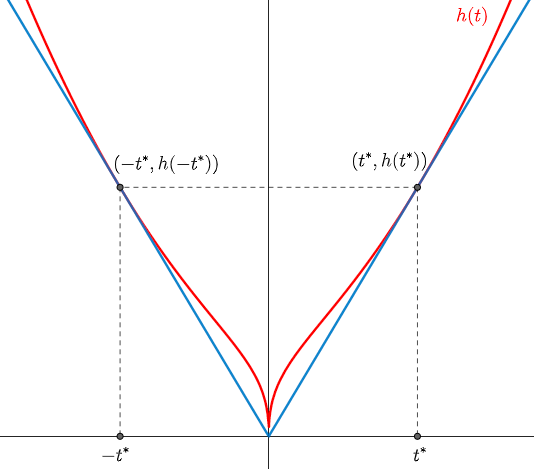
\includegraphics[scale=0.5]{convex.png}
        \caption{The red curve represents the graph of $h$ and the blue lines represents the tangents that pass between $P$ and $(0,0)$ as same as $\tilde{P}$ and $(0,0)$. Notice that for all $t\in \mathbb{R}$, $h(t)$ is over the tangent lines, and for $|t|<t^*$ $h(t)$ is not convex. These facts are important for the construction of the convex envelope of $h$, (see \cite{combettes}) which coincides with the biconjugate of $h$)}
        \label{convex_example}
    \end{figure}  
    
    
    Calling $r^*=\alpha t^*+\beta (t^*)^{q-1}$, we define the function
    \begin{equation}\label{biconjugate}
        \widetilde{h}(t)=\begin{cases}
            h(t),&|t|\ge t^*,\\
            r^*|t|,&|t|<t^*.
        \end{cases}
    \end{equation}
   Then by construction $\widetilde{h}$ is a convex and $C^1$ function except at the origin; moreover, we can check that it is the convex envelope of $h$, so by the Fenchel-Moreau Theorem and Proposition 13.16 of \cite{combettes}, we have that $h^{**}=\widetilde{h}$. The sub differential of this function is given by
   \begin{equation}\label{sub_biconjugate}
       \partial h^{**}(t)=\begin{cases}
           \alpha t+\beta q |t|^{q-1}\sign(t), &|t|\ge t^*,\\                     
           r^*\sign(t), &|t|<t^*, t\ne 0,\\
           [-r^*,r^*], &t=0.
       \end{cases}
   \end{equation}
    We point out that, for each $u\in L^2(\om)$, the integral $\int_{\om}h(u)\; dx$ corresponds to the terms involved with $u$ explicit in the cost function of \eqref{P}. So, since $h^{**}$ corresponds, in its one dimensional version, a convexification of the non convex part present in \eqref{P}, obviously in its one dimensional form, we call the following problem:
    \begin{equation}\label{convex}\tag{$PC_{\lambda}$}
    \begin{cases}
    \displaystyle\min_{(u,y)\in L^2(\om)\times H^1(\Omega)} \;\frac{1}{2}\norm{y-y_d}^2_{L^2(\om)}+\int_{\Omega}h^{**}(u)\; dx\\
    \mbox{subject to:}\\
    Ay(x)=u(x), \phantom{aaaaa} \mbox{in } \om,\\
    \partial_{\Vec{n}}y(x)=0, \phantom{aaaaaaaaaaaaa} \mbox{over } \Gamma,\\    
    y_a\le y(x)+\lambda u(x)\le y(b),\phantom{a} \mbox{almost all }x\in \Omega
    \end{cases}
    \end{equation}
   as the Convex relaxation of \eqref{P}. Notice that this problem has a convex, continuous and bounded-below cost function. These characteristics allow us to prove the following result.
   \begin{lemma}
       Problem \eqref{convex} has a solution.
   \end{lemma}
   \begin{proof}
       Define $J(u)=\frac{1}{2}\norm{Ru-y_d}_{L^2(\Omega)}^2+ \int_{\Omega}h^{**}(u)\, dx$. Let $(u_k,y_k)_{k\in \mathbb{N}}\in L^2(\Omega)\times H^1(\Omega)$ a minimizing and admissible sequence for \eqref{convex}, i.e., the sequence must satisfies that that $u_k=Ry_k$ and 
    \[
    y_a\le y_k(x)+\lambda u_{k}(x)\le y_b,
    \]
    for almost all $x\in \Omega$ and all $k\in \mathbb{N}$. First of all, $(u_k)_{k\in \mathbb{N}}$ forms a bounded sequence, because if it is not, the we can extract a sub-sequence $(u_{k_n})_{n\in \mathbb{N}}$ such that $\norm{u_{k_n}}_{L^2(\Omega)}\to \infty$. But from the definition of $h^{**}$, we have that, if $|t|<t^*$, then $\alpha |t|^2<r^*|t|=h^{**}(t)$. On the other hand, if $|t|\ge t^*$, then $h^{**}(t)=h(t)\ge \frac{\alpha}{2}|t|^2$. So, for every $t\in \mathbb{R}$,
       \[
       h^{**}(t)>\frac{\alpha}{2}|t|^2,
       \]
       witch implies that $\int_{\Omega}h^{**}(u)\; dx>\frac{\alpha}{2}\norm{u}_{L^2(\Omega)}$ and thus $\int_{\Omega}h^{**}(u_{k_n})\; dx\to \infty$. But this contradicts that $(u_k)$ is a minimizing sequence for \eqref{convex}.\\
       
       Now, since $A$ is an elliptic operator, the  Lax Milgram Theorem tell us that $(y_{k})_{k\in \mathbb{N}}$ must be bounded, too, because we known that there exists a constant $c$ depending only of $\Omega$ such that $\norm{y_k}_{H^1(\Omega)}\le c\norm{u_k}_{L^2(\Omega)}$; thereby, the sequence $(y_k,u_k)_{k\in\mathbb{N}}$ forms a bounded sequence in $L^2(\Omega)\times H^1(\Omega)$,  which implies that there must be a sub sequence of $(y_k,u_k)_{k\in\mathbb{N}}$, without renaming, and such that $(y_{k},u_{k})\rightharpoonup (\hat{y},\hat{u})$ in $H^1(\Omega)\times L^2(\Omega)$. However, the weakly convergence of $y_k$ to $\hat{y}$ in $H^1(\Omega)$ implies that $y_{k}\to y$ in $L^2(\Omega)$, and since $y_{k}=Ru_k$, we have that $\hat{y}=R\hat{u}$.\\   

       On the other hand, the weak convergence of $(u_k)$, as same as the strong convergence of $(y_k)$ in $L^2(\Omega)$, implies that for any $\lambda>0$, $y_k+\lambda u_k\rightharpoonup \hat{y}+\lambda\hat{u}$. Since the set
       \[
       L:=\{(w,z)\in L^2(\Omega)\times L^2(\Omega): y_a\le w(x)+\lambda z(x)\le y_b, x\in  \Omega \}
       \]       
       is closed and convex in $ L^2(\Omega)\times L^2(\Omega)$, it must be satisfied that $\hat{y}+\lambda\hat{u}\in L$, proving that the limit points $(\hat{u},\hat{y})$ are also feasible for the problem. Finally, if we call $\hat{J}=\min J(u)$, by the convexity and lower semi continuity of $J$, we have that
       \[
       \hat{J}=\lim_{n\to \infty}J(u_{k_n})\ge \lim\inf_{n\to \infty}J(u_{k_n})\ge J(\hat{u}),
       \]
       and thereby $\hat{u}$ must be a minimize of $J$. Since  $\hat{y}=R\hat{u}$ we have checked that the pair $(\hat{u},\hat{y})$ is a solution for \eqref{convex}.
   \end{proof}\\

    We define the problem $P_0$ as    \begin{equation}\label{P0}\tag{$P_0$}
    \begin{cases}
    \displaystyle\min_{(u,y)\in L^2(\om)\times H^1(\Omega)} \;\frac{1}{2}\norm{y-y_d}^2_{L^2(\om)}+\int_{\Omega}h^{**}(u)\; dx\\
    \mbox{subject to:}\\
    Ay(x)=u(x), \phantom{aaaaa} \mbox{in } \om,\\
    \partial_{\Vec{n}}y(x)=0, \phantom{aaaaaaaaaaaaa} \mbox{over } \Gamma,\\    
    y_a\le y(x)\le y(b),\phantom{aaaaaaaa} \mbox{almost all }x\in \Omega
    \end{cases}
    \end{equation}
    
    Following similar steps of the demonstration of Lemma 1, it is easy to show that this problem has a solution; we note this one as $(\overline{u}, \overline{y})$. Moreover, since the cost function of \eqref{convex} is strictly convex, for each $\lambda>0$ its solution $(u_{\lambda},y_{\lambda})$ is unique. Therefore, if we vary $\lambda$, each solution for \eqref{convex} must vary too. Particularly, we are interested in the sequence of solutions $(\overline{u}_{\lambda}, \overline{y}_{\lambda})$ and its convergence as $\lambda$ tends to zero. The details are the following: defining a positive sequence of reals $(\lambda_n)_{n\in \mathbb{N}}$ tending to zero, and considering the family of problems \eqref{convex_family} defined as
   \begin{equation}\label{convex_family}\tag{$PC_{\lambda_n}$}
    \begin{cases}
    \displaystyle\min_{(u,y)\in L^2(\om)\times H^1(\Omega)} \;\frac{1}{2}\norm{y-y_d}^2_{L^2(\om)}+\int_{\Omega}h^{**}(u)\; dx\\
    \mbox{subject to:}\\
    Ay(x)=u(x), \phantom{aaaaa} \mbox{in } \om,\\
    \partial_{\Vec{n}}y(x)=0, \phantom{aaaaaaaaaaaaa} \mbox{over } \Gamma,\\    
    y_a\le y(x)+\lambda_n u(x)\le y(b),\phantom{a} \mbox{almost all }x\in \Omega
    \end{cases}
    \end{equation}
   we are interested in the relation between $(\overline{u},\overline{y})$ and the sequence of solutions $(\overline{u}_{\lambda_n}, \overline{y}_{\lambda_n})$. The following result shows us this relation.
   
\begin{lemma}
    Consider a sequence of positive scalars $(\lambda_n)_{n\in\mathbb{N}}$ such that $\lambda_n\to 0$ as $n\to \infty$, and the solutions $(\overline{u}_{\lambda_n}, \overline{y}_{\lambda_n})$ of each problem \eqref{convex_family}. Let $(\overline{u},\overline{y})$ the solution of \eqref{P0}. Then, $\overline{u}_{\lambda_n}\to \overline{u}$ strongly in $L^2(\Omega)$.
\end{lemma}

\begin{proof}
Since the cost function in \eqref{convex_family} as same as in \eqref{P0} are strictly convex, and by the compacity and invertibility of the operator $\lambda I+R$, similar arguments presented in Theorem 3.3 in \cite{meyer1} can be followed easly to deduce our result.
\end{proof}\\

Problems \eqref{convex_family} are useful for deducing special features about $ \overline{u}$. We are interested especially in the sparsity of it, because this one will be important for deducing the existence of a solution for \eqref{plambda}. For this purpose, we study the optimal systems constructed for each \eqref{convex_family} and then we investigate the behavior of the limits of each multiplier present in each optimal system as $\lambda$ tends to zero. First of all, we need to compute the sub differenctial of the function $\int_{\om}h^{**}u\; dx$ defined for each $u\in L^2(\om)$, and the following Lemma will be important for this purpose.\\

 \begin{lemma}
    For every $u\in L^2(\Omega)$, we have $h^{**}\circ u\in L^1(\Omega)$.
\end{lemma}
\begin{proof}
    Notice that for $|t|<t^*$,
    \[
    h^{**}(t)<r^*t^*,
    \]
    and for $|t|\ge t^*$, since $2-q>0$, we have that $|t|^{2-q}\ge(t^{**})^{2-q}=2\frac{\beta}{\alpha}(1-q)>\frac{\beta}{\alpha}(1-q)$. This implies that 
    \[
    |t|^{2}>\frac{\beta}{\alpha}(1-q)|t|^q,
    \]
    and finally we have that, for all $t\in \mathbb{R}$,
    \[
    h^{**}(t)<r^*t^*+\left (\frac{\alpha}{2}+\frac{\alpha}{\beta(1-q)}\right)|t|^2.
    \]
    This implies that $h^{**}$ satisfies the conditions (C) and 2.2 of Theorem 2.2 of \cite{ambrosetti}, defining a continuous Nemitski operator from $L^2(\Omega)$ to $L^1(\Omega)$.
\end{proof}\\   


Retaking the question of the desired sub differenctial, if we define $G(u):=\int_{\Omega} h^{**}(u)\; dx$, then by Lemma 3 we have that $\partial G(u)$ is well defined, and
\begin{equation}\label{subdiff_biconjugate}
    \partial G(u):=\{\xi\in L^2(\om): \xi(x)\in \partial h^{**}(u(x)) \mbox{ for almost all }x\in \om \},
\end{equation}
see for example \cite{valkonen}. On the other hand, we can use the artificial control $v=y+\lambda u=$ presented at the beginning of this section for reformulate \eqref{convex_family} as
\begin{equation}\label{reduced}
    \min_{v\in V_{ad}}\frac{1}{2}\norm{SB_{\lambda}v-y_d}^2+\int_{\om}h^{**}(B_{\lambda v}),
\end{equation}
where $V_{ad}=\{v\in L^2(\om): y_a\le v(x)\le y_b, \mbox{ almost all }x\in \om\}$. Since the calculus rules for sub differentials also shows that $\partial G(B_{\lambda}v)=B_{\lambda}^*\partial G(B_{\lambda}v)$ for any $v\in L^{2}\Omega$, Fermat's rule tell us that if $\overline{v}$ is a solution for \eqref{reduced}, then 
\begin{equation}\label{gradient_convex}
0=B^*_{\lambda}(\overline{\phi}+\overline{\zeta})+\overline{\theta},
\end{equation}
where $\overline{\phi}$ satisfies the adjoint equation
\[
\begin{cases}
A^*\overline{\phi}+\overline{\phi}=y-y_d, &\mbox{ in }\Omega,\\
\partial_{\vec{n}}y=0, &\mbox{ over }\Gamma,
\end{cases}
\]
$\overline{\zeta}\in \partial G(B_{\lambda}v)$, and $\theta\in N_{V_{ad}}$, where $N_{V_{ad}}$ stands for the normal cone of $V_{ad}$. Moreover, since $V_{ad}$ has a box-type structure, is well known that the elements of $N_{V_{ad}}$ are characterized by two Lagrange multipliers $\mu_a, \mu_b$ such that \eqref{gradient_convex} can be rearranged as
\begin{equation}\label{gradient_convexII}
B^*_{\lambda}(\overline{\phi}+\overline{\zeta})+\mu_{b}-\mu_a=0,
\end{equation}
with $\mu_a(x), \mu_b\ge 0$ and $\mu_a(x)(v(x)-y_a)=\mu_b(v(x)-y_b)=0$, for almost all $x\in \Omega$. Finally, since $B^{-*}=\lambda I+R^*$, if we apply $B^{-*}$ to \eqref{gradient_convexII}, and using the linearity of $R$, we formulate the following optimally system for \eqref{reduced}:
\begin{align*}
&A\overline{y}+\overline{y}=B_{\lambda}\overline{v}, \qquad \mbox{in }\Omega\\
&\partial_{\vec{n}}\overline{y}=0\qquad\qquad\quad \mbox{over }\Gamma,\\
&A^*\overline{\phi}+\overline{\phi}=y-y_d+\mu_b-\mu_a, \qquad \mbox{in }\Omega\\
&\partial_{\vec{n}}\overline{\phi}=0\hspace{4.25cm}\mbox{over }\Gamma,\\
&\overline{\phi}+\overline{\zeta}+\lambda(\mu_b-\mu_a)=0,\\
&\mu_a, \mu_b\ge 0\\
&\mu_a(\overline{v}-y_a)=\mu_b(\overline{v}-y_b)=0,\\
&\zeta\in \partial G(B_{\lambda}\overline{v})
\end{align*}
Getting back to the original variables $\overline{u}, \overline{y}$ thought the definition of $B_{\lambda}$, and noticing that the problem depends on $\lambda$ we establish the following result.  

\begin{lemma}
    Let $\overline{u}_{\lambda}\in L^{2}(\Omega)$ the optimal control for problem \eqref{convex_family}, and $\overline{y}_{\lambda}$ its associated optimal state. There exists $\overline{\phi}_{\lambda}\in H^1(\Omega)$, $(\mu_a)_{\lambda}, (\mu_b)_{\lambda}, \zeta_{\lambda}\in L^2(\Omega)$ such that the following optimal system is full-filled:    \begin{equation}\label{optimality_convex}
        \begin{cases}         
        A\overline{y}_{\lambda}=\overline{u}_{\lambda}, \qquad \mbox{in }\Omega\\
        \partial_{\vec{n}}\overline{y}_{\lambda}=0\qquad\qquad \mbox{over }\Gamma,\\
        A^*\overline{\phi}_{\lambda}=\overline{y}_{\lambda}-y_d+(\mu_b)_{\lambda}-(\mu_a)_{\lambda}, \qquad \mbox{in }\Omega\\
        \partial_{\vec{n}}\overline{\phi}_{\lambda}=0\hspace{4.25cm}\mbox{over }\Gamma,\\        \overline{\phi}_{\lambda}+\zeta_{\lambda}+\lambda((\mu_b)_{\lambda}-(\mu_a)_{\lambda})=0,\\
        (\mu_a)_{\lambda}, (\mu_b)_{\lambda}\ge 0\\
        (\mu_a)_{\lambda}(\lambda \overline{u}_{\lambda}+\overline{y}_{\lambda}-y_a)=(\mu_b)_{\lambda}(\lambda \overline{u}_{\lambda}+\overline{y}_{\lambda}-y_b)=0,\\
        \zeta_{\lambda}(x)=\begin{cases}
            \alpha \overline{u}_{\lambda}(x)+\beta q |\overline{u}_{\lambda}(x)|^{q-1}\sign(\overline{u}_{\lambda}(x)), &|\overline{u}_{\lambda}(x)|>t^*\\
            r^*\sign(\overline{u}_{\lambda}(x)), &|\overline{u}_{\lambda}(x)|\le t^*, |\overline{u}_{\lambda}(x)|\ne 0,\\
            \nu \in [-r^*,r^*],& |\overline{u}_{\lambda}(x)|=0
        \end{cases}  
        \end{cases}
    \end{equation}    
\end{lemma}
\begin{proof}
    We have discussed that $\zeta_{\lambda}\in L^2(\Omega)$ by properties of the sub differentials of functions of the form of $G$. Since $\overline{\phi}_{\lambda}$ is the solution of the adjoint equation $A\overline{\phi}_{\lambda}+\overline{\phi}_{\lambda}=\overline{y}_{\lambda}-y_d$, we have $\overline{\phi}_{\lambda}\in L^2(\om)$, so $\overline{\phi}_{\lambda}+\zeta_{\lambda} \in L^2(\Omega)$. Finally, from the characterization of the elements from the normal cone to $V_{ad}$ and by the box-type structure of this set, we take $((\mu_a)_{\lambda})=[B_{\lambda}^*(\overline{\phi}_{\lambda}+\overline{\zeta}_{\lambda})]_+$ and $(\mu_a)_{\lambda}=[B_{\lambda}^*(\overline{\phi}_{\lambda}+\zeta_{\lambda})]_-$, being $[\cdot]_{+}$ and $[\cdot]_-$ the positive and negative parts of theirs arguments. This shows us the regularity of $(\mu_a)_{\lambda}, (\mu_b)_{\lambda}$ and the gradient equation $\overline{\phi}_{\lambda}+\zeta_{\lambda}+\lambda((\mu_b)_{\lambda}-(\mu_a)_{\lambda})=0$. The complementary conditions $(\mu_a)_{\lambda}(\lambda\overline{u}+\overline{y}-y_a)=(\mu_b)_{\lambda}(\lambda\overline{u}+\overline{y}-y_b)=0$ follows from the box structure of $V_{ad}$, since is a well know result (see for example \cite{delosreyes}) that if $\overline{\phi}\in L^2(\om), \zeta\in L^{\infty}(\om), \overline{w}\in L^2(\om)$ are optimal solutions for $(PC_{\lambda})$, then
\[
    \overline{v}(x)=\mathcal{P}_{[y_a,y_b]}(\overline{v}(x)-c\mu(x)),
\]
 where $\overline{v}=B_{\lambda}^{-1}\overline{u}$. Finally, the explicit form of $\zeta_{\lambda}$ follows from \eqref{sub_biconjugate} and \eqref{subdiff_biconjugate}.
\end{proof}\\

Notice that the optimal system above depends on $\lambda$; therefore, we want to know what happens with the multipliers $\overline{\phi}_{\lambda}, (\mu_a)_{\lambda}, (\mu_b)_{\lambda}$ and $\zeta_{\lambda}$ as $\lambda\to 0$. The limits of each multiplier are important to construct a solution for the original problem \eqref{plambda}. The following theorem show us the structure of these limits.
\begin{theorem}
    Let $(\overline{u}_n)_{n\in\mathbb{N}}$ the sequence of optimal controls for each $(PC_{\lambda_n})$, where $(\lambda_n)_{n\in \mathbb{N}}$ is a sequence of positive reals such that converges to $0$. Let suppose that the measure of the set $\Omega_{0}:=\{x\in \om: |\overline{u}(x)|=0\}$ is zero. Consider the multipliers $\overline{\phi}_n, \zeta_{n}, (\mu_a)_n, (\mu_b)_n$ that appears for each optimal system $(PC_{\lambda_n})$ according to Lemma 4. Then exists $\mu_a, \mu_b\in L^2(\om)$ such that $(\mu_a)_n\rightharpoonup \mu_a, (\mu_b)_n\rightharpoonup \mu_b$, there exists a sub sequence of $(\zeta_n)$ which converges strongly to $\zeta\in L^2(\Omega)$ defined as
    \[
    \zeta(x)=\begin{cases}
        \alpha \overline{u}(x)+\beta q |\overline{u}(x)|^{q-1}\sign(\overline{u}(x)), &|\overline{u}(x)|>t^*\\
            r^*\sign(\overline{u}(x)), &|\overline{u}(x)|\le t^*,
    \end{cases}
    \] 
    and exist $\overline{\phi}\in L^2(\om)$ such that $\overline{\phi_n}\to \overline{\phi}$ strongly in $L^2(\Omega)$, where $\overline{\phi}=R^*(\overline{y}-y_d+\mu_b-\mu_a)$.
\end{theorem}
\begin{proof}
Since $\overline{u}_n\to \overline{u}$ strongly in $L^2(\om)$ we know that there exists a bounded sub sequence $(u_{n_k})_{k\in\mathbb{N}}$ such that $\overline{u}_{n_k}(x)\to \overline{u}(x)$ almost all $x\in \om$; thereby, $\lambda_n \overline{u}_{n_k}(x)\to 0$. On the other hand, by the continuity of $R$ we must have again that there exists a sub sequence of $(y_{n_k})_{k\in \mathbb{N}}$ such that $\overline{y}_{n_k}(x)\to \overline{y}(x)$ almost all $x\in \om$. This implies that, for almost all $x\in \Omega$,
\begin{equation}\label{subseq}
\lambda\overline{u}_{n_k}(x)+\overline{y}_{n_k}(x)-y_a\to \overline{y}(x)-y_a,
\end{equation}
almost all $x\in \om$. Now, by contradiction suppose that $((\mu_a)_n)_{n\in \mathbb{N}}$ is unbounded. Then, there must exists a sub sequence of $((\mu_a)_{n_k})_{k\in\mathbb{N}}$ such that $\norm{(\mu_a)_{n_k}}\to\infty$. The last relation implies that for almost all $x\in \Omega$, $(\mu_a)_{k_n}(x)\to \infty$, because if not, there must be a positive constant $M$ such that $(\mu_a)_{n_k}(x)\le M$ for all $k\in\mathbb{N}$ and almost all $x\in \om$. But then
\[
\int_{\om}(\mu_a)_{n_k}(x)^2\;dx\le M^2|\om|,
\]
for all $k$, contradicting that $\norm{(\mu_a)_{n_k}}\to\infty$. Now, from the seventh equation of $(PC_{\lambda})$ we have that, for all $n\in\mathbb{N}$ and almost all $x\in \Omega$,
\begin{equation}\label{subseqII}
(\mu_a)_n(x)(\lambda_n\overline{u}_n(x)+\overline{y}_n(x)-y_a)=0,
\end{equation}
and the last equation follows for the sub sequences $(\overline{u}_{n_k}), (\overline{y}_{n_k})$ and $((\mu_a)_{n_k})$, too. Since the last equation must follows for almost all $x\in \Omega$, there must be satisfied for almost all $x$ such that $\overline{y}-y_a\ne 0$. But from \eqref{subseq} we have that $\lambda\overline{u}_{n_k}(x)+\overline{y}_{n_k}(x)-y_a$ cannot converge to zero. Since $\overline{u}_{n_k}(x)\to \infty$, we cannot have \eqref{subseqII} for all $k\in \mathbb{N}$, and thereby the optimal system is not full-filled, contradicting our main hypothesis.\\

Similar arguments can be used for proving that the sequence $((\mu_b)_n)_{n\in\mathbb{N}}$ is bounded in $L^2(\Omega)$; hence, there must exist $\mu_a, \mu_b\in L^2(\Omega)$ such that $(\mu_a)_{n}\rightharpoonup \mu_a$ and $(\mu_b)_{n}\rightharpoonup \mu_b$. Now, since $\overline{\phi}_{n}=R^{*}(\overline{y}_n-y_d+(\mu_b)_n-(\mu_a)_n)$ and $R$ is a compact embedding from $L^2(\om)$ to itself, then $\overline{\phi}_{n}\to \overline{\phi}$ strongly in $L^2(\om)$, where $\overline{\phi}=R^*(\overline{y}-y_d+\mu_b-\mu_a)$.\\

Finally, from \eqref{subdiff_biconjugate} we know that $\zeta_n\in L^2(\Omega)$ for all $n\in \mathbb{N}$. As we have exposed before, there exist a uniformly bounded sub sequence of $(u_n)$ such that $\overline{u}_{n_k}(x)\to \overline{u}(x)$. On the other hand, notice that $h^{**}(t)$ is a $C^1$ function over $\mathbb{R}\setminus\{0\}$, with derivate
\[
(h^{**})'(t)=\begin{cases}
    \alpha t+\beta q |t|^{q-1}\sign(t), &|t|>t^*\\
            r^*\sign(t), &|t|\le t^*,
    \end{cases}
\]
Moreover, for all $t\in\mathbb{R}\setminus\{0\}$
\[
(h^{**})'(t)\le r^{*}+(\alpha+\beta q(t^{*})^{q-1})|t|,
\]
so, by continuity of $(h^{**})'$ we have that $(h^{**})'(\overline{u}_{n_k}(x))\to (h^{**})'(\overline{u}(x))$. The Dominated Convergence Theorem concludes the desired result.
\end{proof}\\

\begin{remark}
From the last Theorem and the fifth equation of $(PC_{\lambda})$ plus the boundedness of $(\mu_{a})_{n}$ and $(\mu_{b})_{n}$ we can extract a sub sequence of $(\zeta)_{n}$ and a sub sequence of $(\overline{\phi})_n$ such that
\[
0=\lim_{n\to \infty}((\overline{\phi})_n(x)+(\zeta)_{n}(x)+\lambda((\mu_{b})_{n})-(\mu_{a})_{n})=\overline{\phi}(x)+\zeta(x),
\]
almost all $x\in \Omega$. This implies that for almost all $x$ where $|\om_0|=0$ that $\overline{\phi}(x)=-\zeta(x)$. This will be useful for the next Theorem.
\end{remark}


The last Theorem of this section is devoted to prove the existence of at least one non trivial solution for \eqref{plambda}. 

\begin{theorem}
    Let $(\overline{u}_{n})_{n\in \mathbb{N}}$ the sequence associated to the optimal system $(PC_{\lambda_n})$, where $(\lambda_n)_{n\in \mathbb{N}}$ is a sequence of positive reals tending to zero. Also, suppose that if $|\overline{u}_{n}(x)|\le t^*$, then $\overline{u}_{n}(x)=0$. The limit $\overline{u}$ of this sequence is an optimal solution for \eqref{P}, with associated state $\overline{y}=R\overline{u}$.
\end{theorem}

\begin{proof}
   It is easy to prove that the limit of the sequence $(\overline{u}_n)$ must satisfies almost everywhere that if $|\overline{u}(x)|\le t^*$, then $\overline{u}=0$. Now, we can see that
    \begin{align*}
        J(y,u)-J(\overline{y},\overline{u})=&(\overline{y}-y_d, R(u-\overline{u}))_{L^2(\Omega)}+\alpha(u-\overline{u},u)_{L^2(\Omega)}\\
        &+\frac{1}{2}\norm{y-\overline{y}}_{L^2(\om)}^2+\frac{\alpha}{2}\norm{u-\overline{u}}_{L^2(\om)}^2\\
        &+\beta\left(\int_{\Omega}|u(x)|^q\; dx-\int_{\om}|\overline{u}(x)|\; dx\right)
    \end{align*}
    From the continuity of $R$, the scalar product and the optimal system $(PC_{\lambda_n})$, we have
    \begin{align*}
        (\overline{y}-y_d, R(u-\overline{u}))_{L^2(\Omega)}&=\lim_{k\to \infty}(\overline{y}_{n_k}-y_d, R(u-\overline{u}_{n_k}))_{L^2(\om)}\\
        &=\lim_{k\to \infty}(\overline{\phi}_{n}+R^*((\mu_{a})_n-(\mu_{b})_n), u-\overline{u}_{n_k}))_{L^2(\om)}\\
        &=(\overline{\phi},(u-\overline{u}))_{L^2(\om)}+(\mu_a-\mu_b,y-\overline{y})_{L^2(\om)}.
    \end{align*}
    First of all, notice that $\mu_a, \mu_b\ge 0$. On the other hand, the weakly convergence of $(\mu_a)_{n}$ plus the uniform convergence of $(u_{n})$ and the seventh equation of $(PC_{\lambda})$ implies that $(\mu_a,y_a-\overline{y})_{L^2(\om)}=0$. Thereby
    \begin{align*}
    (\mu_a,y-\overline{y})_{L^2(\om)}&=\lim_{n\to\infty}[(\mu_a)_{n},y-y_a)_{L^2(\om)}+((\mu_a)_{n},y_a-\overline{y})_{L^2(\om)}]\\
    &= (\mu_a,y-y_a)_{L^2(\om)}+(\mu_a,y_a-\overline{y})_{L^2(\om)}\\
    &\ge 0.
    \end{align*}
    A similar analysis show us that $-(\mu_b,y-\overline{y})_{L^2(\om)}\ge 0$. These two last facts implies that
     \begin{align*}
        J(y,u)-J(\overline{y},\overline{u})\ge&(\overline{\phi}+\alpha \overline{u},u-\overline{u})_{L^2(\Omega)}\\
        &+\frac{1}{2}\norm{y-\overline{y}}_{L^2(\om)}^2+\frac{\alpha}{2}\norm{u-\overline{u}}_{L^2(\om)}^2\\
        &+\beta\left(\int_{\Omega}|u(x)|^q\; dx-\int_{\om}|\overline{u}(x)|^q\; dx\right)
    \end{align*}
    Take $\om_1=\{x\in \om: |\overline{u}(x)|>t^*\}$, and $\om_2=\{x\in \om: |\overline{u}(x)|<t^*, \overline{u}(x)\ne 0\}$; in the first case, by Remark 1 we have that $\overline{\phi}(x)=-\alpha\overline{u}(x)-\beta q|\overline{u}|^{q-1}\sign(\overline{u}(x))$. Taking account of these fact, we have that over $\om_1$
    \begin{align*}
        (\overline{\phi}+\alpha \overline{u},u-\overline{u})_{L^2(\Omega)}+&\beta\left(\int_{\Omega}|u(x)|^q\; dx-\int_{\om}|\overline{u}(x)|^q\; dx\right)\\
        &=\beta\int_{\om_1}[q|\overline{u}|^{q-1}\sign(\overline{u}(x))][\overline{u}(x)-u(x)(x)]+|u(x)|^q-|\overline{u}(x)|^q\; dx
    \end{align*}
    Using a second order Taylor expansion of $|{u}(x)|^q$ around $\overline{u}(x)$, we have that the last integral is equal to
    \[
    \int_{\om_1}\frac{\beta}{2}q(q-1)|\overline{u}(x)|^{q-2}(u(x)-\overline{u}(x))^2\; dx+o(|u(x)-\overline{u}(x)|^2)
    \]
    Since $o(|u(x)-\overline{u}(x)|^2)\ge 0$ and $|\overline{u}(x)|>t^*$, we have that
    \begin{equation}\label{om1}
        (\overline{\phi}+\alpha \overline{u},u-\overline{u})_{L^2(\Omega)}+\beta\left(\int_{\Omega}|u|^q\; dx-\int_{\om}|\overline{u}|^q\; dx\right)\\>-q\frac{\alpha}{2}\int_{\om_1}(u(x)-\overline{u}(x))^2\; dx
    \end{equation}
    On the other hand, we have that for almost all $x\in \om_2$, $\overline{\phi}(x)=-r^*\sign(\overline{u}(x)$. This implies that over this set
    \begin{align*}
        (\overline{\phi}+\alpha \overline{u},u-\overline{u})_{L^2(\Omega)}+&\beta\left(\int_{\Omega}|u|^q\; dx-\int_{\om}|\overline{u}|^q\; dx\right)\\
        &=\int_{\om_1}[\alpha\overline{u}-r^*\sign(\overline{u})][u-\overline{u}]+\beta(|u|^q-|\overline{u}|^q)\; dx.\\
        &\ge \int_{\om_1}[\alpha\overline{u}-r^*\sign(\overline{u})][u-\overline{u}]-\beta|\overline{u}|^q)\; dx\\
        &\ge-\frac{\alpha}{2}\int_{\om_2}(u-\overline{u})^2 \, dx+\int_{\om_2}r^*\sign(\overline{u})[\overline{u}-u]-\beta|\overline{u}|^q\; dx\\
        &\ge -\frac{\alpha}{2}\int_{\om_2}(u-\overline{u})^2 \, dx+\int_{\om_2}r^*\sign(\overline{u})[\overline{u}-u]-\beta|\overline{u}|^q\; dx.
    \end{align*}
    But, since $\overline{u}(x)=0$ over the set $\om_2$, we finally have that 
    \begin{equation}\label{om2}
        (\overline{\phi}+\alpha \overline{u},u-\overline{u})_{L^2(\Omega)}+\beta\left(\int_{\Omega}|u|^q\; dx-\int_{\om}|\overline{u}|^q\; dx\right)\ge -\frac{\alpha}{2}\int_{\om_2}(u-\overline{u})^2 \, dx
    \end{equation}
    Therefore, by \eqref{om1} and \eqref{om2} we have that
    \begin{align*}
        J(y,u)-J(\overline{y},\overline{u})\ge&\left[(\overline{\phi}+\alpha\overline{u},u-\overline{u})_{L^2(\Omega)}+\beta\left(\int_{\Omega}|u(x)|^q\; dx-\int_{\om}|\overline{u}(x)|\; dx\right)\right]\\
        &+\frac{1}{2}\norm{y-\overline{y}}_{L^2(\om)}^2+\frac{\alpha}{2}\norm{u-\overline{u}}_{L^2(\om)}^2\\
        >&\left[-q\frac{\alpha}{2}\int_{\om_1}(u-\overline{u})^2\; dx-\frac{\alpha}{2}\int_{\om_2}(u-\overline{u})^2 \, dx\right]\\
        &+\frac{\alpha}{2}\int_{\om_1}(u-\overline{u})^2\; dx+\frac{\alpha}{2}\int_{\om_2}(u-\overline{u})^2\; dx\\
        =&(1-q)\frac{\alpha}{2}\int_{\om_1}(u-\overline{u})^2\; dx\ge 0,
    \end{align*}
    and thus $\overline{u}$ is a solution for $\eqref{P}$, with state $\overline{y}=R\overline{u}$.
\end{proof}\\

\subsection{Application to a non convex optimal control problem with pure point-wise state constrains}

The last result is useful for the study of the following optimal control problem: letting $\Omega, \Gamma$ as same as the problem \eqref{plambda}, $A$ the same elliptic operator as this problem, $a_{ij}, a_0$ the same functions, $\alpha, \beta>0$ and $q\in ]0,1[$, we consider the problem
\begin{equation}\label{P}\tag{P}
    \begin{cases}
    \displaystyle\min_{(y,u)\in H^1(\om)\times L^2(\om)}\; \frac{1}{2}\norm{y-y_d}^2_{L^2(\om)}+\frac{\alpha}{2}\norm{u}^2_{L^2(\om)}+\beta \int_{\om} |u|^{q}\; dx\\
    \mbox{subject to:}\\
    Ay(x)=u(x), \phantom{aaa} \mbox{in } \om,\\
    \partial_{\Vec{n}}y(x)=0, \phantom{aaaaaaaaaaa} \mbox{over } \Gamma,\\    
    y_a\le y(x)\le y_b,\phantom{aaaaaaal} \mbox{almost all }x\in \Omega
    \end{cases}
\end{equation}

This problem is interesting in practical situations, due to the non convex penalty and the pure point-wise state constraints: for example in problems that demands sparcity over the optimal control, and for which the state must be bounded point wise. However, the study of this problem directly could result difficult because the lack of convexity in the cost function, as same as the point-wise state constrains; two paradigms that are being discussed widely before. However, all the previous work can be applied for investigating solutions for this problem. Firs of all, from \eqref{P} we can introduce a \textit{Lavrentiev regularization} of the point-wise state constrains, which consist in replacing the point-wise state constrains of \eqref{P} by the mixed restriction $y_a\le y(x)+\lambda u(x)\le y_b$, obtaining the problem \eqref{plambda}. It was shown in Theorem 2. that this problem has a solution $\overline{u}$ which is the limit of the sequence of optimal controls $(\overline{u}_{\lambda_n})_{n\in\mathbb{N}}$ which satisfies the optimal system \eqref{optimality_convex}. Under the same assumptions of Theorem 2 for $\overline{u}$, plus the strong convergence of $(\overline{u}_{\lambda_n})_{n\in\mathbb{N}}$ to $\overline{u}$ as $\lambda \to 0$, we must have that the sequence of associated states $(y_{\lambda_n})_{n\in\mathbb{N}}$ converges strongly to the state $\overline{y}=R\overline{u}$. The compacity of $R$ and the strong convergence of $(\overline{u}_{\lambda_n})_{n\in\mathbb{N}}$ and $(\overline{y}_{\lambda_n})_{n\in\mathbb{N}}$ shows that $(\overline{u}, \overline{y})$ are feasible for \eqref{P}. Finally, the structure of $\overline{u}$ allow us to follow the following result
\begin{theorem}
    Let $\overline{u}$ satisfiying the hypothesis of Theorem 2. Then, $\overline{u}$ is a solution for \eqref{P} with associated state $\overline{y}=R\overline{u}$.
\end{theorem}


\section{DC-Optimal System for problem \eqref{plambda}}

In this section we develop an optimal system for the studied problem \eqref{plambda}, using a technique presented in \cite{merino} known as \textit{Huber regularization}. The main purpose behind this is to reformulate \eqref{plambda} as the difference of two convex functions and then, thanks to the DC-theory, to formulate first order necessary conditions which will be useful for the numerical treatment of the problem. 

\subsection{Huber regularization for the non convex term of \eqref{plambda}}
For $q\in ]0, 1[$ and $\gamma>>1$, we introduce the following function:
\[
h_{q,\gamma}(t)=\begin{cases}
q\gamma^{\frac{1-q}{q}}|t|^{\frac{1}{q}}, & |t|\le \frac{1}{\gamma},\\ 0, & \mbox{otherwise.} 
\end{cases}
\]
defined for all $t\in \mathbb{R}$. Then, for each $u\in L^2(\om)$ we define the mapping
\[
\Upsilon_{q,\gamma}(u)=\int_{\om}h_{q,\gamma}(u(x))^q\; dx,
\]
which is called a \textit{Huber-type regularization} for the quasi norm $\int_{\om}|u|^q\; dx$ present in \eqref{P}.
 With this new function, we formulate the following optimal control problem based on \eqref{plambda}:
\begin{equation}\tag{$PH_{\lambda}$} \label{phuber}
    \begin{cases}
    \displaystyle\min_{(y,u)\in H^1(\om)\times BV(\om)} \frac{1}{2}\norm{y-y_d}^2_{L^2(\om)}+\frac{\alpha}{2}\norm{u}^2_{L^2(\om)}+\beta\Upsilon_{q,\gamma}(u)\\
    \mbox{subject to:}\\
    Ay(x)=u(x), \phantom{aaaa} \mbox{in } \om,\\
    \partial_{\Vec{n}}y(x)=0, \phantom{aaaaaaaaaaaa} \mbox{over } \Gamma,\\
   y_a\le\lambda u(x)+y(x)\le y_b, \phantom{aaa} \mbox{a.e in }\om 
    \end{cases}
\end{equation}
As same as the previous Section, if we define the artificial control $v=(\lambda I+R)u$, for any $u\in L^2(\om)$, and if we introduce the indicator function (see Section 2), \eqref{phuber} can be reformulated as 
\[
	\begin{cases}
		\displaystyle \min_{v\in L^{2}(\om)} \qquad  \frac{1}{2}\norm{S	B_{\lambda}v-y_d}_{L^2(\om)}^2+\frac{\alpha}{2}\norm{	B_{\lambda}v}_{L^2(\om)}^2+\beta\Upsilon_{q,\gamma}(	B_{\lambda}v)+\mathbf{I}_{V_{ad}}(v),
		\end{cases}
\]
where $ V_{ad}:=\{v\in L^2(\om): y_a\le v(x)\le y_b, \mbox{ a.e }x\in K\subset\subset\om \}$. Now, for every $v\in L^2(\om)$ we set 
\begin{equation}\label{convexI}
	F(v):=\frac{1}{2}\norm{S	B_{\lambda}v-y_d}_{L^2(\om)}^2+\frac{\alpha}{2}\norm{	B_{\lambda}v}_{L^2(\om)}^2+\beta\kappa_{\gamma}\norm{B_{\lambda}v}_{L^{1}(\om)}+\mathbf{I}_{V_{ad}}(v),
\end{equation}
and
\begin{equation}\label{convexII}
	G(v):=\beta \l(\kappa_{\gamma}\norm{B_{\lambda}v}_{L^{1}(\om)}-\Upsilon_{p,\gamma}(B_{\lambda}v)\r).
\end{equation}
Clearly, the reduced problem can be stated as
\begin{equation}\label{1}
    	\min_{v\in L^2(\om)} F(v)-G(v).
\end{equation}
Notice that $F$ is convex, because it is composed by the sum of $L^1$ and $L^2$ norms, plus the indicator function which is obviously convex. On the other hand, it can be shown (see Lemma 5 of \cite{merino}) that $G$ is convex too; therefore, the last optimal control problem \eqref{1} can be regarded as a problem of difference of convex functions.\\

We point out that the function
 \[
        t\mapsto \kappa_{\gamma}|t|-h_{q,\gamma}(t),
    \]
is Gâteaux differentiable (see Lemma 6 of \cite{merino}), with derivate
 \begin{equation}\label{j}
        j(t)=\begin{cases}
            \kappa_{\gamma}-q\l(|t|+\dfrac{q-1}{\gamma}\r)^{q-1}\sign(t), & \mbox{if }|t|\ge \frac{1}{\gamma},\\
            0, &\mbox{if not},
        \end{cases}
    \end{equation}
    and moreover, from the linearity and invertibility of $B_{\lambda}$ for small enought $\lambda$ and the Gâteaux differentiability of $h_{q,\gamma}$, we get the Gâteaux differentiability of $G(B_{\lambda}v)$ for each $v\in V_{ad}$.\\
    
 Previous the deduction of the optimal system for \eqref{phuber}, we present some results. The next result allow us to well define the subdifferential of $\int_{\om} h^{**}(u)\; dx$ for each $u\in L^2(\om)$.

 From the theory of Difference of Convex functions (DC-theory, see for example \cite{dihn, merino})  we know that if $\overline{v}$ is a solution for \eqref{1}, we have 
\begin{equation}\label{opt}
    \partial G(\overline{v})\subset\partial F(\overline{v}),
\end{equation}
where $F, G$ are the two convex functions defined in \eqref{convexI} and \eqref{convexII}. So, the main objective in this part is to characterize the sub differentials for $F$ and $G$ respectively. For this purpose, consider
\[
	f(v):=\frac{1}{2}\norm{S	B_{\lambda}v-y_d}_{L^2(\om)}^2+\frac{\alpha}{2}\norm{	B_{\lambda}v}_{L^2(\om)}^2,
\]
for all $v\in L^2(\om)$. It can be easily checked that $f$ is Fréchet differentiable, with derivate 
\[\nabla f(\overline{v})=B_{\lambda}^*(\overline{\phi}+\alpha B_{\lambda}\overline{v}),
\]
and $\overline{\phi}$ the adjoint state solution to the equation 
\[
\begin{cases}
A^*\phi+\phi=y-y_{d}, &\mbox{in }\om\\
\partial_{\vec{n}}\phi=0,&\mbox{over }\Gamma
\end{cases}
\]
Calling 
\begin{equation}\label{zeta}
	\zeta(x)=\begin{cases}
		1, & \mbox{almost all }x\in \om \mbox{ such that } B_{\lambda}v(x)>0,\\
		-1, & \mbox{almost all }x\in \om \mbox{ such that }B_{\lambda}v(x)<0\\
		\mu \in [-1,1], &\mbox{almost all }x\in \om \mbox{ such that } B_{\lambda}v(x)=0,
	\end{cases}
\end{equation}
then, from \eqref{opt} and the theory of convex analysis (see for example \cite{rock}) we deduce the following result. 
 \begin{lemma}  
     If $\overline{v}$ is a solution of \eqref{opt}, there exists $\overline{w}\in L^2(\om)$, $\overline{\phi}\in H^1(\om)$, $\zeta\in L^{\infty}(\om)$ y $\theta \in N_{V_{ad}}$ such that     
     \begin{equation}\label{gradiente1}
         \beta B_{\lambda}^*\overline{w}=B_{\lambda}^*(\overline{\phi}+\alpha B_{\lambda}\overline{v})+\beta\kappa_{\gamma}B_{\lambda}^*\zeta+\theta,
     \end{equation}
     where $N_{V_{ad}}$ stands for the normal cone to $V_{ad}$.
\end{lemma}

Now, from the characterization of the normal cones presented, for example in \cite{rock}, we can deduce the following.
\begin{theorem} 
	If $\overline{v}$ is a solution for \eqref{opt}, then there exists $\overline{y}\in H^1(\om)$, $\overline{w}\in L^2(\om)$, $\overline{\phi}\in H^1(\om)$, $\zeta\in L^\infty(\om)$ such that the following optimal conditions are full-filled
	\begin{equation}\label{optii1}
    \begin{split}
	&A\overline{y}=B_{\lambda}\overline{v}, \\
	&\partial_{\vec{n}} y=0, \\
	&A^*\overline{\phi}+\overline{y}-y_d=0,\\
	&\partial_{\vec{n}}\overline{\phi}=0,\\
	&(B_{
	\lambda}^*(\overline{\phi}+\alpha B_{\lambda}\overline{v}+\beta( \kappa_{\gamma}\zeta-w)),\nu-\overline{v})_{L^2(\om)}\ge 0, \;\mbox{ for almost all }\nu \in V_{ad},\\
	&\zeta(x)=\begin{cases}
		1, & \mbox{almost all }x\in \om \mbox{ such that } B_{\lambda}v(x)>0,\\
		-1, & \mbox{almost all }x\in \om \mbox{ such that }B_{\lambda}v(x)<0\\
		\mu \in [-1,1], &\mbox{almost all }x\in \om \mbox{ such that } B_{\lambda}v(x)=0,
	\end{cases}\\
	&w-j(B_{\lambda}\overline{v})=0.
\end{split}
\end{equation}
\end{theorem}

\begin{proof}
 It is a well-know fact that, if $Y$ is a convex cone, then its normal cone $N_{Y}$ is characterized as
\[
    N_{Y}(x)=\partial \mathbf{I}_{Y}(x)=\{x^*\in X^*:\langle x^*, \tilde{x}-x\rangle_{X^*,X}\le 0,  \mbox{ for all }\tilde{x}\in Y\}.
\]
See, for example \cite{rock}. So, using the Riesz representative of $B_{
	\lambda}^*(\overline{\phi}+\alpha B_{\lambda}\overline{v}+\beta( \kappa_{\gamma}\zeta-w))$ and using the same nottion for it, then the gradient equation \eqref{gradiente1} is converted into the presented form in the optimal system presented above.
\end{proof}\\

The next theorem allow us to rewrite the last optimal system in terms of the originals state and control $y, u$, and introducing two $L^{2}(\om)$ Lagrange multipliers which they allow us to rewrite the gradient inequality presented above.

\begin{lemma}
Let $\overline{u}\in L^2(\om)$ the optimal control state of \eqref{plambda}. Then, there exists $\overline{y}, \overline{\phi}\in H^1(\om)$, $\mu_a,\mu_b, \overline{w}\in L^2(\om)$, $\zeta\in L^{\infty}(\om)$ such that the following KKT system is full filled:
%\newpage
\begin{equation}\label{opti3}
\begin{split}
	&A \overline y=\overline{u}, \qquad\qquad\qquad\qquad \; \mbox{in }\om,\\
	&\partial_{\vec{n}} y=0, \qquad\qquad\qquad\qquad\qquad \mbox{over }\Gamma,\\
	&A^*\overline{\phi}+\overline{y}-y_d-\mu_{b}+\mu_{a}=0,\quad \;\;\mbox{in }\om,\\
	&\partial_{\vec{n}}\overline{\phi}=0,\qquad\qquad\qquad\qquad\qquad \mbox{over }\Gamma,\\
	&\overline{\phi}+\alpha \overline{u}+\beta( \kappa_{\gamma}\zeta-\overline{w})+\lambda( \mu_b- \mu_a)=0,\\
	&\mu_{a}, \mu_{b}\ge 0,\\
	&\mu_{a}(\lambda\overline{u}+\overline{y}-y_a)=\mu_{b}(B_\lambda\overline{u}+\overline{y}-y_b)=0,\\
    &\overline{w}-j(\lambda u+y)=0
\end{split}
\end{equation}
and
\[
\zeta(x)=\begin{cases}
		1, & \mbox{a.a. }x\in \om \mbox{ such that } \overline{u}(x)>0,\\
		-1, & \mbox{a.a. }x\in \om \mbox{ such that } \overline{u}(x)<0,\\
		\mu \in [-1,1], &\mbox{a.a. }x\in \om \mbox{ such that } \overline{u}
  \end{cases}
\]
\end{lemma}

\begin{proof}
    Calling 
    \[
    \mu_a=[B_{\lambda}^*(\overline{\phi}+\alpha B_{\lambda}\overline{v}+\beta\kappa_{\gamma}\zeta-w)]_{+},\qquad
    \mu_b=[B_{\lambda}^*(\overline{\phi}+\alpha B_{\lambda}\overline{v}+\beta\kappa_{\gamma}\zeta-w)]_{-}, 
\]
it can be followed similar arguments used in Lemma 4 to prove the non negativity and regularity of multipliers $\mu_a, \mu_b$, as well as the complementary conditions that must be satisfied. Finally, if $\overline{v}$ is the solution of \eqref{plambda}, and since $B_{\lambda}\overline{v}=\lambda\overline{y}+\overline{u}$, we can replace all $B_{\lambda}\overline{v}$ terms in \eqref{optii1} with  $B_{\lambda}\overline{v}=\lambda\overline{y}+\overline{u}$, concluding the result. 
\end{proof}


\section{DC-Semi-smooth Newton Method}

In this section we propose a numerical solution scheme based on Semi-smooth Newton algorithm (\cite{merino1, ulbrich}). First we define two funtions $C_1:L^2(\om)\times H^{1}(\om)\times L^2(\om)\to L^2(\om)$ and $C_2:L^2(\om)\times L^{\infty}(\om)\to L^2(\om)$, defined as
\[
    C_{1}(\mu,y,u)=\mu-\max(0,c_1(\lambda u+y-y_b)+\mu)+\min(0,c_1(\lambda u+y-y_a)+\mu),
\]
and
\[
C_{2}(u.\zeta)=u-\max(0,u+c_2\kappa_{\gamma}\beta(\zeta-1))-\min(0,u+c_2\kappa_{\gamma}\beta(\zeta+1)).
\]
with these two functions, we can easily verify that the optimal system \eqref{opti3} can be rewrite as

\begin{subequations}\label{1.6}
\begin{align}
    &E\overline{y}-\overline{u}=0,\subtag{a}\\
    &E^*\overline{\phi}-\overline{y}+y_d+\mu=0,\subtag{b}\\
    &\overline{\phi}+\alpha \overline{u}+\beta (\kappa_{\gamma}\zeta-w)+\lambda \mu=0,\subtag{c}\\
    &C_1(u,y,\mu)=0,\subtag{d}\\
    &C_2(u,\zeta)=0,\subtag{e}\\
    &w-j(u)=0,\subtag{f}
\end{align}
\end{subequations}
where $E$ denotes the differential operator associated to the P.D.E that rules the optimal control problem. The following result proves that the left hand sides of \eqref{1.6} can define a semi smooth function (see \cite{ulbrich}).

\begin{lemma}
The function $j$ introduced in \eqref{j} defines a continuous Nemitski  operator from $L^2(\om)$ to $L^2(\om)$.
\end{lemma}

\begin{proof}
Clearly, the function $j$ is a continuous function over $\reals$. Now, if $|t|\le \frac{1}{\gamma}$, $j(t)=0$, so for all constants $a,b>0$ we have $j(t)<a+b|t|$. Suppose that $|t|>\frac{1}{\gamma}$. Then we have
\[
    |j(t)|\le \kappa_{\gamma} +q\l||t|+\frac{q-1}{\gamma}\r|^{q-1}.
\]
Now,
\[
|t|>\frac{1}{\gamma}\Rightarrow |t|+\frac{q-1}{\gamma}>\frac{q}{\gamma}
\]
and since $\gamma>1>q$, we have
\[
    \l(|t|+\frac{q-1}{\gamma}\r)^{1-q}<\l(\frac{q}{\gamma}\r)^{1-q}.
\]
This implies that
\[
|j(t)|<\kappa_{\gamma}+q\l(\frac{q}{\gamma}\r)^{1-q}.
\]
If we define $a=\kappa_{\gamma}+q\l(\frac{q}{\gamma}\r)^{1-q}$, then, clearly
\[
|j(t)|\le a+|t|.
\]
Therefore, the conditions (C) and 2.2 established for continuous Nemintski operators in \cite{ambrosetti} are full-filled, and our result follows from Theorem 2.2 in \cite{ambrosetti}. 
\end{proof}




\begin{theorem}
\normalfont
    Let $E=H^1(\om)\times L^{2}(\om)\times L^{2}(\om)\times L^{2}(\om)\times L^{\infty}(\om)\times L^{2}(\om)$ and $\mathcal{F}: E\to E$ a function with variables $\overline{y},\overline{u},\overline{\phi},\mu,\zeta,w$ defined by the left hand sides of \eqref{1.6}. Then, $\mathcal{F}$ is semi smooth
\end{theorem}
\begin{proof}
For each $u \in L^2(\om)$, define $Tu=S^*(S(u)-y_d)$. Then, we have $\overline{y}=S\overline{u}$, $\overline{\phi}=T\overline{u}$ and $w=j(u)$. from equation c in \eqref{1.6}, it follows that
\[
    \kappa_{\gamma}\beta\zeta=\beta j(u)-\lambda \mu-T\overline{u}-\alpha\overline{u}.
\]
Define 
\[
    \mathcal{F}_1(u,\mu)=\mu-\max(0,c_1(\lambda u+Su-y_b)+\mu)-\min(0,c_1(\lambda u+Su-y_a)+\mu),
\]
\begin{align*}
    \mathcal{F}_2(u,\mu)=&u-\max(0,u+c_2(\beta j(u)-\lambda\mu-Tu-\alpha u-\kappa_{\gamma}\beta))\\
    &-\min(0,u+c_2(\beta j(u)-\lambda\mu-Tu-\alpha u+\kappa_{\gamma}\beta)),
\end{align*}
so $\mathcal{F}(\cdot)=0$ is equivalent to $\mathcal{F}_1(\cdot)=0$ and $\mathcal{F}_2(\cdot)=0$. If we proof that both $\mathcal{F}_1$ and $   \mathcal{F}_2$ are semi smooth, then we can conclude the semi smoothnes of $\mathcal{F}$.


If $c_1=\frac{1}{\lambda}$ we have that
\[
    \mathcal{F}_1(u,\mu)=\mu-\max\l(0,u+\frac{1}{\lambda}Su-\frac{1}{\lambda} y_b+\mu\r)-\min\l(0,u+\frac{1}{\lambda}Su-\frac{1}{\lambda}y_a+\mu\r),
\]
otherwise, if  $c_2=\frac{1}{\alpha}$, we have that
\begin{align*}
    \mathcal{F}_2(u,\mu)=&u-\frac{\beta}{\alpha}\bigg[\max\l(0,j(u)-\frac{\lambda }{\beta}\mu-\frac{1}{\beta}Tu-\kappa_{\gamma}\r)\\
    &-\min\l(0,j(u)-\frac{\lambda }{\beta}\mu-\frac{1}{\beta}Tu+\kappa_{\gamma}\r)\bigg].
\end{align*}
Now, notice that $\mathcal{F}_1$ has the term $M(u,\mu)=u+\frac{1}{\lambda}Su+\mu+c$, which $c$ a constant that could be $-\frac{1}{\lambda}y_a$ or $-\frac{1}{\lambda}y_b$. Since $S$ is a continuous linear operator, clearly $M$ is Fréchet differentiable for any $(u,\mu)\in L^2(\om)^2$. Finally, is a well-known fact that $\max(0,\cdot)$ and $\min(0,\cdot)$ are semi smooth functions are (see for example \cite{delosreyes} o \cite{ito-kunish}). Moreover, the composition of a Fréchet differentiable function with a semi smooth function results in a semi smoot function, proving that $\mathcal{F}_1$ is semi smooth. A similar analysis can be done for proving that $\mathcal{F}_2$ is also a semi smooth function. 
\end{proof}\\

We know (see for example\cite{ulbrich, meyer1, stadler}) that the Semi-smooth Newton type methods are useful for the numerical resolution of the equation
\begin{equation}\label{SSN}
     \mathcal{F}(x)=0,
\end{equation}   

especially when $\mathcal{F}$ is a semi-smooth function. The main idea of the method is the following: given $x^k$, $k\in \mathbb{N}$, the next iteration of SSN method (semi-smooth Newton method) $x^{k+1}$ must satisfies the equation
\[
F(x^k)+\mathcal{G}(x^k)(x^{k+1}-x^k)=0,
\]
where $\mathcal{G}$ denotes the generalized derivate of $\mathcal{F}$. In our case, the generalized derivate has the form 
\begin{equation}
    \mathcal{G}(p)=\begin{pmatrix}
    E               &0      &   -I                  &0                       &0                                           &0\\
    -I              &E      &   0                   &I                       &0                                           &0\\
    0               &I      & \alpha I              &\lambda I               &\beta\kappa_{\gamma}I                       &-\beta I\\
    \chi_{A}        &0      & \lambda(\chi_{A})     &c_1\lambda(I-\chi_{A})    &0                                           &0\\
    0               &0      &   I-\chi_{\tilde{A}}  &0                       &-c_2\kappa_{\gamma}\beta(\chi_{\tilde{A}})    &0\\
    0               &0      &   j'(u_k)             &0                       &   0                                        &-I
    \end{pmatrix}
\end{equation}

with 
\[
    A_1=\{x: c_1(\lambda u+y-y_b)+\mu\ge 0\}, A_2=\{x: c_1(\lambda u+y-y_a)+\mu \le 0\}, A=A_1\cup A_2,
\]
\[
    A_3=\{x:u+c\kappa_{\gamma}\beta(\zeta-1)\ge 0\},  A_4=\{x:u+c\kappa_{\gamma}\beta(\zeta+1)\le 0\},  \tilde{A}=A_3\cup A_4.
\]
Our semi-smooth algorithm is based over similar models proposed, for example in \cite{ulbrich, stadler, meyer1} and many other literature steps. Specifically, the algorithm used in this paper is summarized as follows:  \\

\textbf{Algorithm 1}
\begin{enumerate}
    \item 
    Take $\epsilon>0$, a initial point $p_0=(\overline{y}_0,\overline{\phi}_0,\overline{u}_0,\overline{\mu},\overline{\zeta}_0,\overline{w}_0)$ sufficiently close to the solution of \eqref{SSN} $k=0$ and $\delta_{k}$ appropriately chosen for checking the condition $\norm{d_k}>\epsilon$.    
    \item
       While $\norm{\delta_{p_k}}\ge \epsilon$:
        \begin{enumerate}
            \item 
            Compute $F(x_k)$, $F'(p_k)$ and find $\delta_{p_{k}}$ from the system
            \[
                F'(p_k)\delta_{p_{k}}=-F(p_k)
            \]
            \item
                Take
                \[
                    p_{k+1}=p_k+\delta_{p_k}
                \]
            \item
                Set $\delta_{p_{k+1}}=p_{k+1}-p_{k}$ and compute $\norm{\delta_{p_{k+1}}}$. 
            \end{enumerate}
        \item
        If $\norm{\delta_{p_{k+1}}}\ge \epsilon$, then go to step 2, setting $k=k+1$.  Otherwise, stop the algorithm and take $p_{k+1}$ as the solution for \eqref{SSN}.
\end{enumerate}

The stopping criteria is based on the next argument: since we expect that the the sequence of $(p_n)$ satisfies $\lim_{k\to\infty}\mathcal{F}(p_k)=0$,
the residual $\delta_{p_{n}}$ should tends to zero as $k\to \infty$. The following theorem allow us to expect the convergence of our algorithm to a solution for \eqref{SSN}.

\begin{theorem}
    The algorthim 1 converges to the solution of problem  if $x^0$ is sufficiently close to this solution  
\end{theorem}

\begin{proof}
    We know that $\mathcal{F}$ is a semi-smooth function, so, by Theorem 9 of \cite{stadler}, it is sufficient to prove that $\mathcal{G}$ has a bounded inverse. The inversibility of $\mathcal{G}$ follows from the following facts: first of all, the elliptic operator used in out problem admitis for each $z\in L^2(\om)$ a unique $\overline{\varphi}\in H^1(\om)$ such that $E\varphi=z$. The same holds for $E^*$. Finally, the dependence of the multipliers $\mu, \xi$, as same as the adjoint state, only of the optimal control and state for \eqref{P} follows the fact that there exist only one solution for the equation 
    \[
    \mathcal{G}(X)=Y,
    \]
    where $X,Y\in E$, and $E$ defined as in Theorem 7, and therefore $\mathcal{G}$ is invertible. Finally, the continuity of $E$ and $E^*$, plus the structure of the active sets follows by the Bounded Inverse Theorem that $\mathcal{G}^{-1}$ is bounded, and thereby the Newton semi-smooth method will converge to a solution of the problem.    
\end{proof}


\section{Numerical results}

The optimal control problem that we consider for testing our results is the following: setting $\om=[0,1]^2$, we formulate the problem:

\begin{equation}
    \begin{cases}
    \displaystyle\min_{(y,u)\in H^1(\om)\times L^2(\om)}\; \frac{1}{2}\norm{y-y_d}^2_{L^2(\om)}+\frac{\alpha}{2}\norm{u}^2_{L^2(\om)}+\beta \int_{\om} |u|^{q}\; dx\\
    \mbox{subject to:}\\
    -\Delta y+y=u, \phantom{aaa} \mbox{in } \om,\\
    \partial_{\Vec{n}}y(x)=0, \phantom{aaaaa} \mbox{over } \Gamma,\\    
    -1\le y(x)\le 0.2 ,
    \end{cases}
\end{equation}
where 
\[
    y_d(x_1,x_2)=\left(x_1-\frac{1}{2}\right)^2+\left(x_2-\frac{1}{2}\right)^2,
\]
for all $(x_1,x_2)\in [0,1]^2$. For the discretization of the domain and the numerical approximation of the integrals we use a finite difference scheme: using the standar partition of the domain into $n^2$ equidistant nodes $(x_1^i,x_2^j)$ for $i,j=1,\cdots,n$, with $x_1^i=\frac{i}{n+1}$ and $x_2^j=\frac{j}{n+1}$.\\

Setting $h=\frac{1}{n+1}$, we use the following midpoint rule for calculating the double integrals that appear in the problem:

\begin{align*}
    \int_{a}^{b}\int_{c}^{d}u(x_1,x_2)\; dx_2\;dx_1\approx& \frac{1}{4}h^2\Bigg[ u(a,c)+u(b,c)+u(a,d)+u(b,d)\\
    &\phantom{aaaa} +2\sum_{i=1}^{n-2}u(x_i,c)+2\sum_{i=1}^{n-2}u(x_i,d)+2\sum_{i=1}^{n-2}u(a,y_i)\\
    &\phantom{aaaa}+2\sum_{i=1}^{n-2}u(b,y_i)+4\sum_{i=1}^{n-2}\sum_{i=1}^{n-2}u(x_i,y_j)\Bigg]
\end{align*}
The evaluations of $u$ in each node $[(x_1^i, x_2^j)]_{i,j=1}^n$ is structured in a vector $\mathbf{U}\in \reals^{n^2}$; thereby, the $L^1(\Omega)$ norm of $u$ is aproximated as
\[    \norm{u}_{L^1(\Omega)}\approx\sum_{i=1}^{n^2}c_i|\mathbf{U}_i|,
\]
where each $c_i$ is calculated through the midpoint formula presented above. Moreover, the discretization of the PDE presented in our numerical example produces a linear system of the form $(LAP+I_{n^2})Y=U$, where $Y\in \mathbb{R}^{n^2}$ are the discretization of $y$ into each node $(x_1^i,x_2^j)$, and $LAP$ is the matrix defined as
\[
   \mbox{LAP}=\frac{1}{h^2} \begin{pmatrix}
    A&-I_n&\\
    -I_n&B&-I_n\\
    &-I_n&B&-I_n\\
    &&\ddots&\ddots&\ddots\\
    &&&&B&-I_n\\
    &&&&-I_n&A
    \end{pmatrix}_{n^2\times n^2},
\]
where
\[
    A=\begin{pmatrix}
    2&-1\\
    -1&3&-1\\
      &-1&3&-1\\
      &&\ddots&\ddots&\ddots\\
      &&-1&3&-1\\
      &&&-1&2
    \end{pmatrix}_{n\times n}, \qquad B=\begin{pmatrix}
    3&-1\\
    -1&4&-1\\
      &-1&4&-1\\
      &&\ddots&\ddots&\ddots\\
      &&-1&4&-1\\
      &&&-1&3
    \end{pmatrix}_{n\times n}.
\]
We point out that the matrices above defined came from the classical formulae of the Laplacian into finite differences. At first experiment we take $\alpha=1e-2$, $\beta=2e-4$ and $q=\frac{1}{2}$. The regularization parameter has the values $\lambda=1e-4$ and $\gamma=2500$; additionally, we take $c_1=100$ and $c_2=50$ in the semi-smooth algorithm. For the discretization of the unit square we have considered a partition of $100\times 100$ internal nodes. The program that we use to the numerical experiments is Matlab R2021a. The graphics of the change of the residual in each iteration, such as the variation of the cost are presented in the following image:
\begin{figure}[h]
    \centering
    \begin{minipage}{0.5\textwidth}
        \centering
        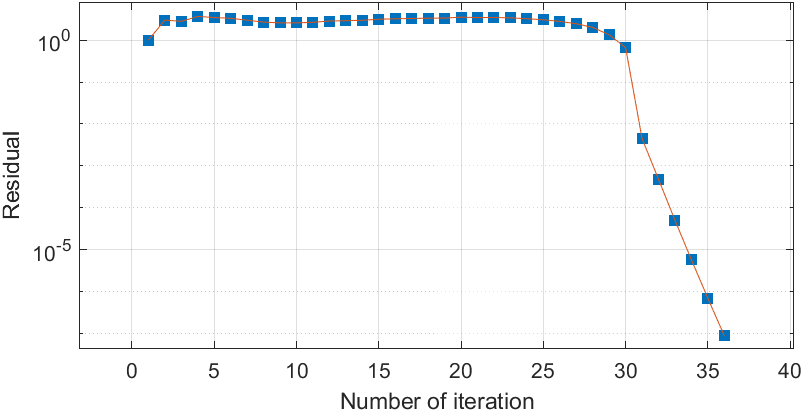
\includegraphics[width=1\textwidth]{residual.png} % first figure itself      
    \end{minipage}\hfill
    \begin{minipage}{0.5\textwidth}
        \centering
        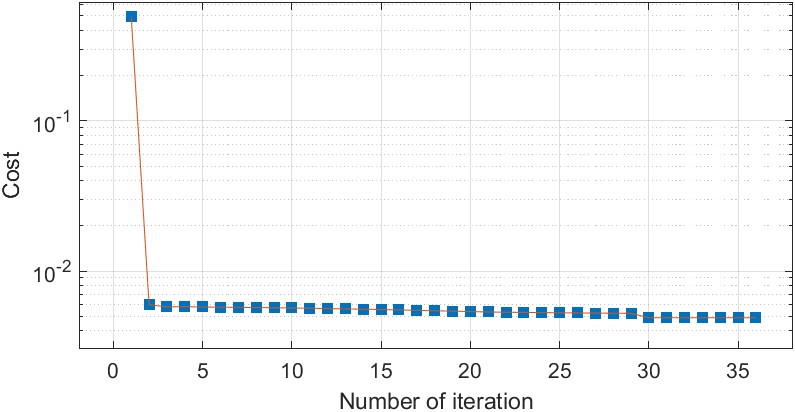
\includegraphics[width=1\textwidth]{cost.png} % second figure itself        
    \end{minipage}
    \caption{Residual and Cost of the problem vs number of iterations of the algorithm}
\end{figure}

   We can appreciate that, despite the convergence of the algorithm, the residual behavior tends to have low variations until the thirtieth iteration, where the residual descends significantly. On the other hand, the cost of the problem tends to stabilize before the fifth iteration. Table 1. presents a summarize of the numerical evolution of our algorithm through the 35 iterations. We point out that until the iteration number $25$, the residual tends to decrease slowly. However, the number of null elements of the optimal control $u$ tends to increase until a stabilization. As null elements of u we refer to the entries $u(\cdot,\cdot)$ which are small enough to be considerate as zero.

\begin{table}[h]
    \centering
    \begin{tabular}{|c|c|c|c|c|}
    \hline
    It. &Null elements in $u$ &Residual     & Cost\\ 
    \hline
1  & 0    & 3.0087     & 0.005972\\  
2  & 1696 & 2.7933     & 0.005772  \\
3  & 776  & 3.6731     & 0.0057934 \\
4  & 2520 & 3.4509     & 0.0057655 \\
5  & 2708 & 3.3105     & 0.0057486 \\
10 & 3244 & 2.658      & 0.0056555 \\
15 & 3808 & 3.2191     & 0.00551   \\
20 & 4452 & 3.4425     & 0.0053416 \\
25 & 4804 & 2.7981     & 0.0052616 \\
30 & 4876 & 0.0044843  & 0.0048893 \\
31 & 4876 & 0.00047814 & 0.0048893 \\
32 & 4876 & 5.0666e-05 & 0.0048893 \\
33 & 4876 & 5.735e-06  & 0.0048893 \\
34 & 4876 & 6.9444e-07 & 0.0048893 \\
35 & 4876 & 8.8643e-08 & 0.0048893 \\
    \hline
\end{tabular}
\caption{Numerical results of the experiment incorporated.}
\end{table}
\subsection{Varying problem parameters} In this section we present the results of varying individually the parameters $\alpha, \beta$ and $q$ present in \eqref{P}. In the first case, we vary only $\alpha$, taking $\beta=2e-3$, $p=2$, $\lambda=1e-4$ and $\gamma=2500$. Table 2 summarizes our results:
\begin{table}[h]
    \centering
    \begin{tabular}{|c|c|c|c|c|}
    \hline
    $\alpha$ & Optimal cost & Null elements in $u$ & Number of iterations\\
    \hline
    0.0175&0.0055555&4796&49\\
    0.0125&0.0053958&6076&43\\
    0.01  & 0.0052986 &6676  & 43  \\
    0.005 &0.0050413 &7900  &44\\
    0.003 &0.0048888 &8460  &45\\
    0.00125 & 0.0046883 & 9056 & 47\\
    \hline
    \end{tabular}
    \caption{Variations of $\alpha$}
\end{table}

Notice that, as $\alpha$ decrease, the null elements in $u$ tends to increase and the number of iterations are relatively constant. Next, we vary $\beta$, taking $\alpha=0.0175$, $p=2$, $\lambda=1e-4$ and $\gamma=2500$. Results are summarized in the Table 3.
\begin{table}[h]
    \centering
    \begin{tabular}{|c|c|c|c|c|}
    \hline
    $\beta$ & Optimal cost & Null elements in $u$ & Number of iterations\\
    \hline
    0.00125&0.0053617&4192&44\\
    0.0007&0.0052083&3684&40\\
    0.00025  & 0.0050747 &3028  & 37  \\
    0.000075&0.0050198&2556&35\\
    5e-5&0.0050099&1788&35\\
    1e-5 &0.0049953 &496  &60\\
    1e-6 &0.0049921 &88  &37\\    
    \hline
    \end{tabular}
    \caption{Variations of $\beta$}
\end{table}

The effect that we report over the sparsity of $u$ in this case is the opposite of the previous case: here, as $\beta$ tends to decrease, the null elements in $u$ tends to decrease too. Finally, we vary the parameter $p$, taking $\alpha=0.01, \beta=3e-4, \lambda=1e-4$ and $\gamma=2500$. The results are summarized in Table 4.
\begin{table}[h]
    \centering
    \begin{tabular}{|c|c|c|c|c|}
    \hline
    $p$ & Optimal cost & Null elements in $u$ & Number of iterations\\
    \hline
    1.1&00.0048639&1196&42\\
    1.4&0.0048828&3012&37\\
    2&0.0049158&5144&37\\
    3.5  & 0.0049367 &5392  & 37  \\
    5&0.0049464&5336&38\\
    5.2&0.0049477&5296&38\\   
    \hline
    \end{tabular}
    \caption{Variations of $p$}
\end{table}

We notice that, as $p$ tends to increase, the sparcity of $u$ tends to increase too. The number of iterations again are relatively constant, and in general, the optimal cost in each reported cases tends to present small variations during the variation of the parameters. The graphical solutions of each group of experiments, as its graphical supports are presented in Figures 3, 4 and 5.\\

\subsection{Varying regularization parameters}
In this sub section we report our numerical experiments at which the regularization parameters are tested, keeping fixed the parameters of the problem. The main idea of this section is to observe the behavior of the optimal control as $\gamma$ tends to infinity and $\lambda$ tends to zero. First of all, we present the numerical results of varying $\gamma$, keeping $\alpha=0.01, \beta=0.0003, p=2$ and $\lambda=1e-4$.  Results are summarized in Table 5.  
\begin{table}[h].
    \centering
    \begin{tabular}{|c|c|c|c|c|}
    \hline
    $\gamma$ & Optimal cost & Null elements in $u$ & Number of iterations\\
    \hline
    1500&0.0049158&5144&37\\
    3500&0.0049158&5144&37\\
    6000&0.0049158&5144&37\\
    10000  & 0.0049158 &5144  & 37  \\
    1e5&0.0049158&5144&37\\ 
    \hline
    \end{tabular}
    \caption{Varations of $\gamma$}
\end{table}

\begin{figure}[H]
    \centering
    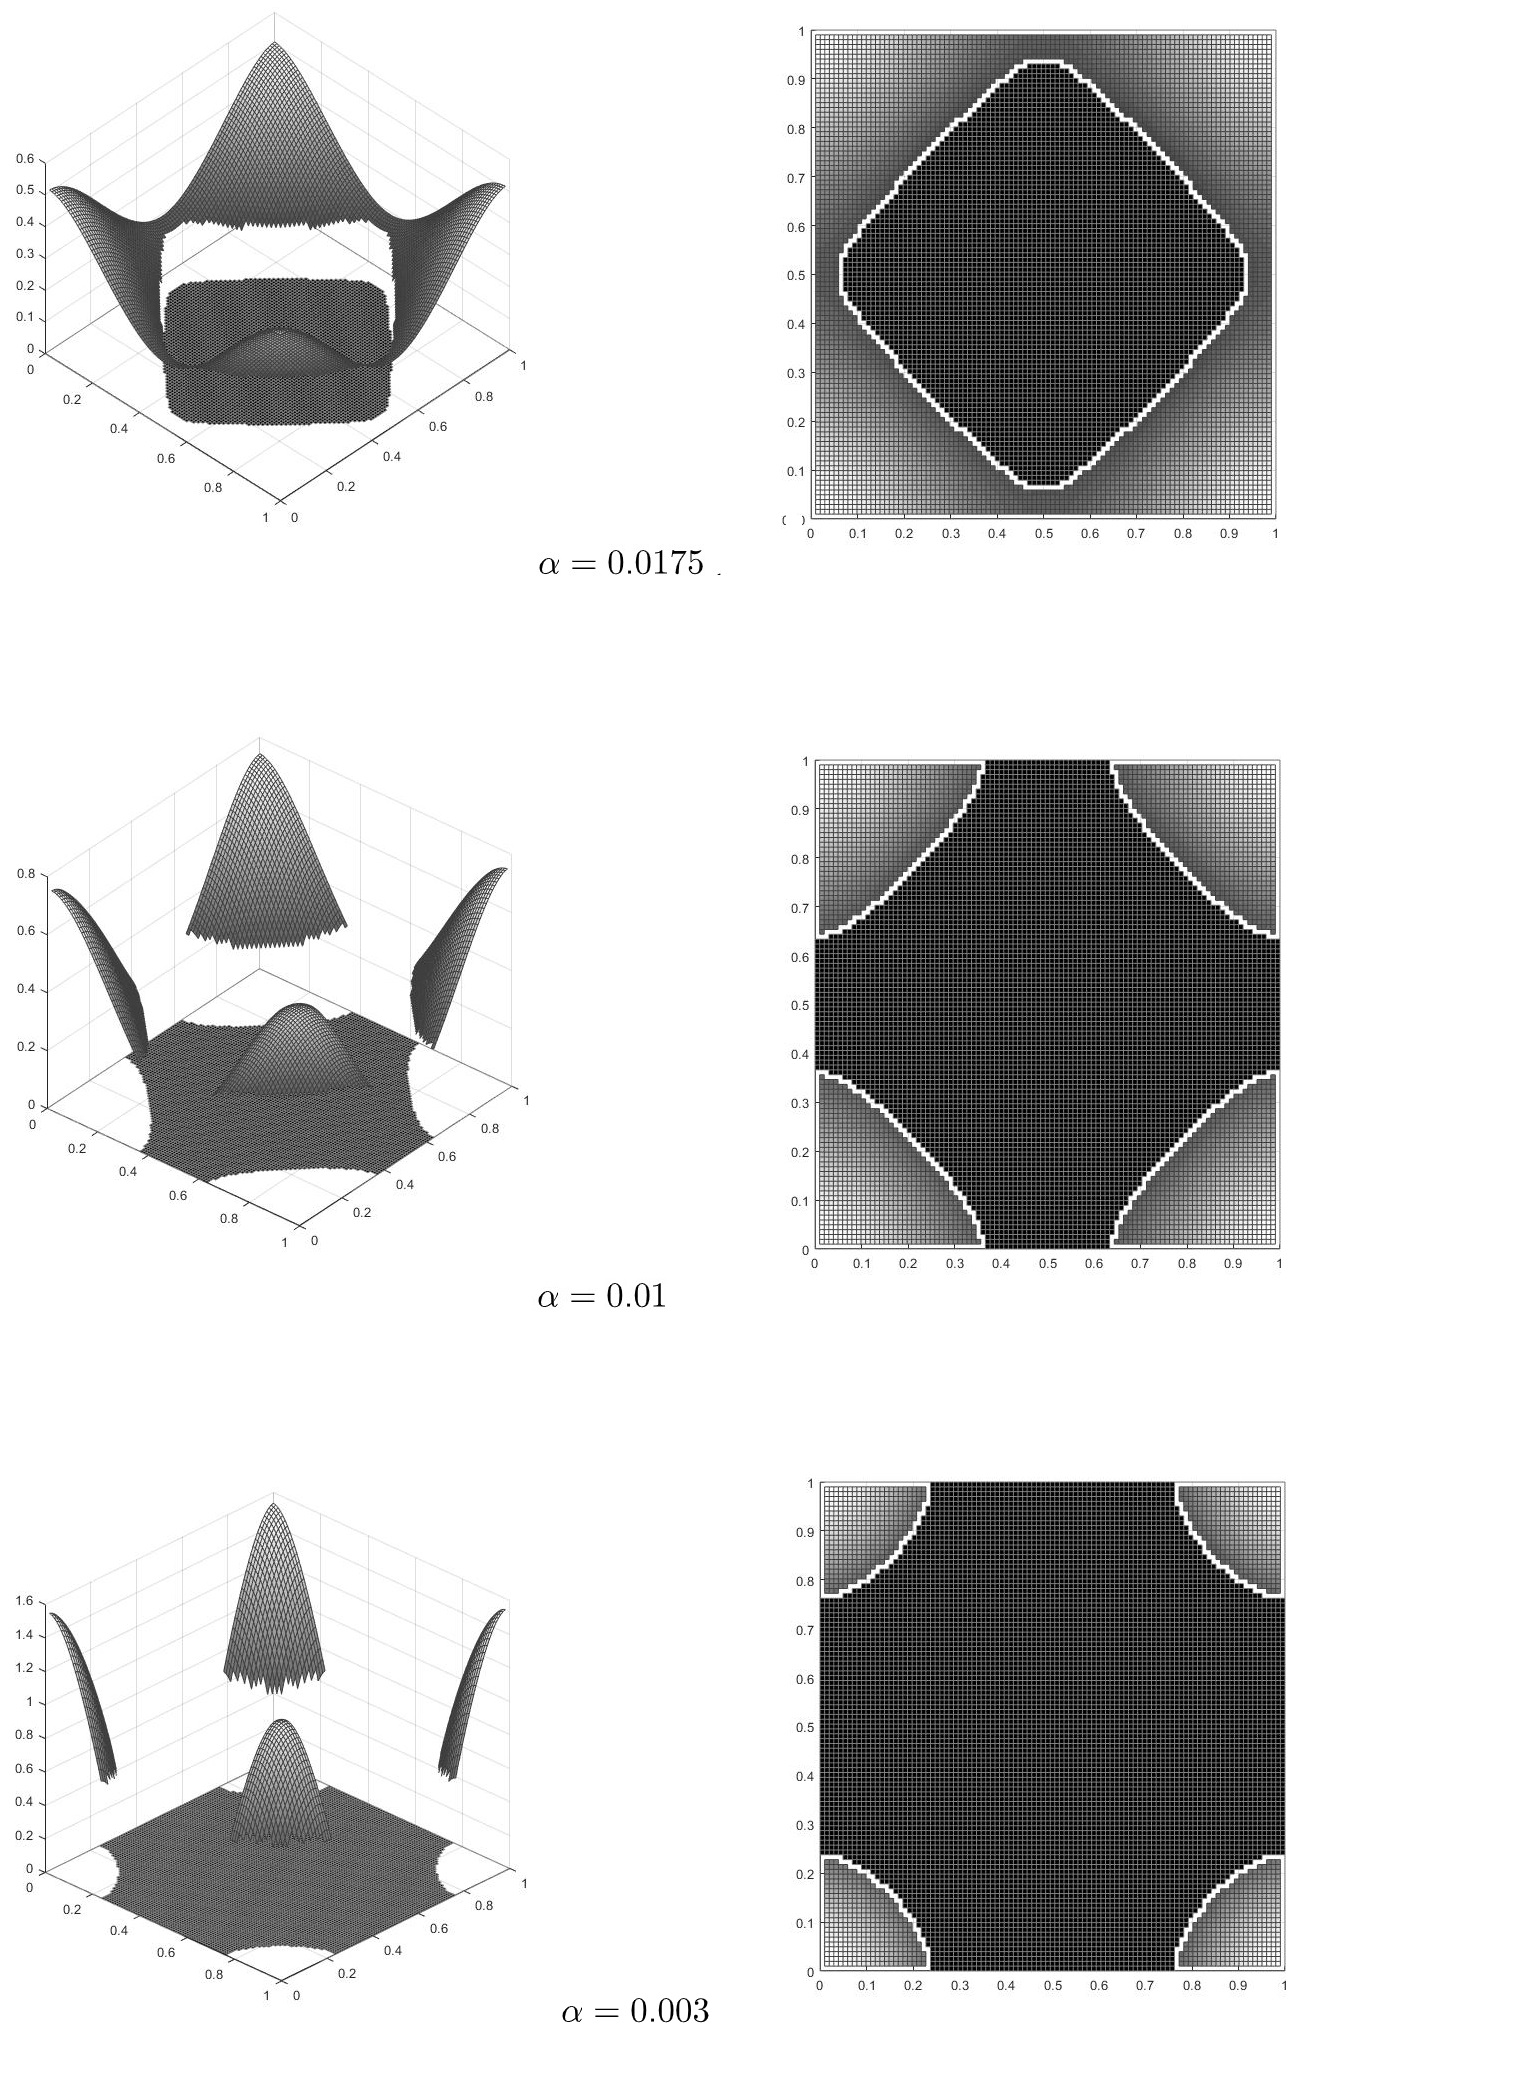
\includegraphics[scale=0.35]{matrizaa.jpg}
    \caption{Graphics of the optimal control $u$ (first column) and their supports (second column) as $\alpha$ varies. The first row correspond to the solution when $\alpha=0.0175$, the second corresponds to $\alpha=0.01$ and third corresponds to $\alpha=0.003$. We notice that, as $\alpha$ decrease, the support of function decrease, too.}
\end{figure}




\begin{figure}[H]
    \centering
    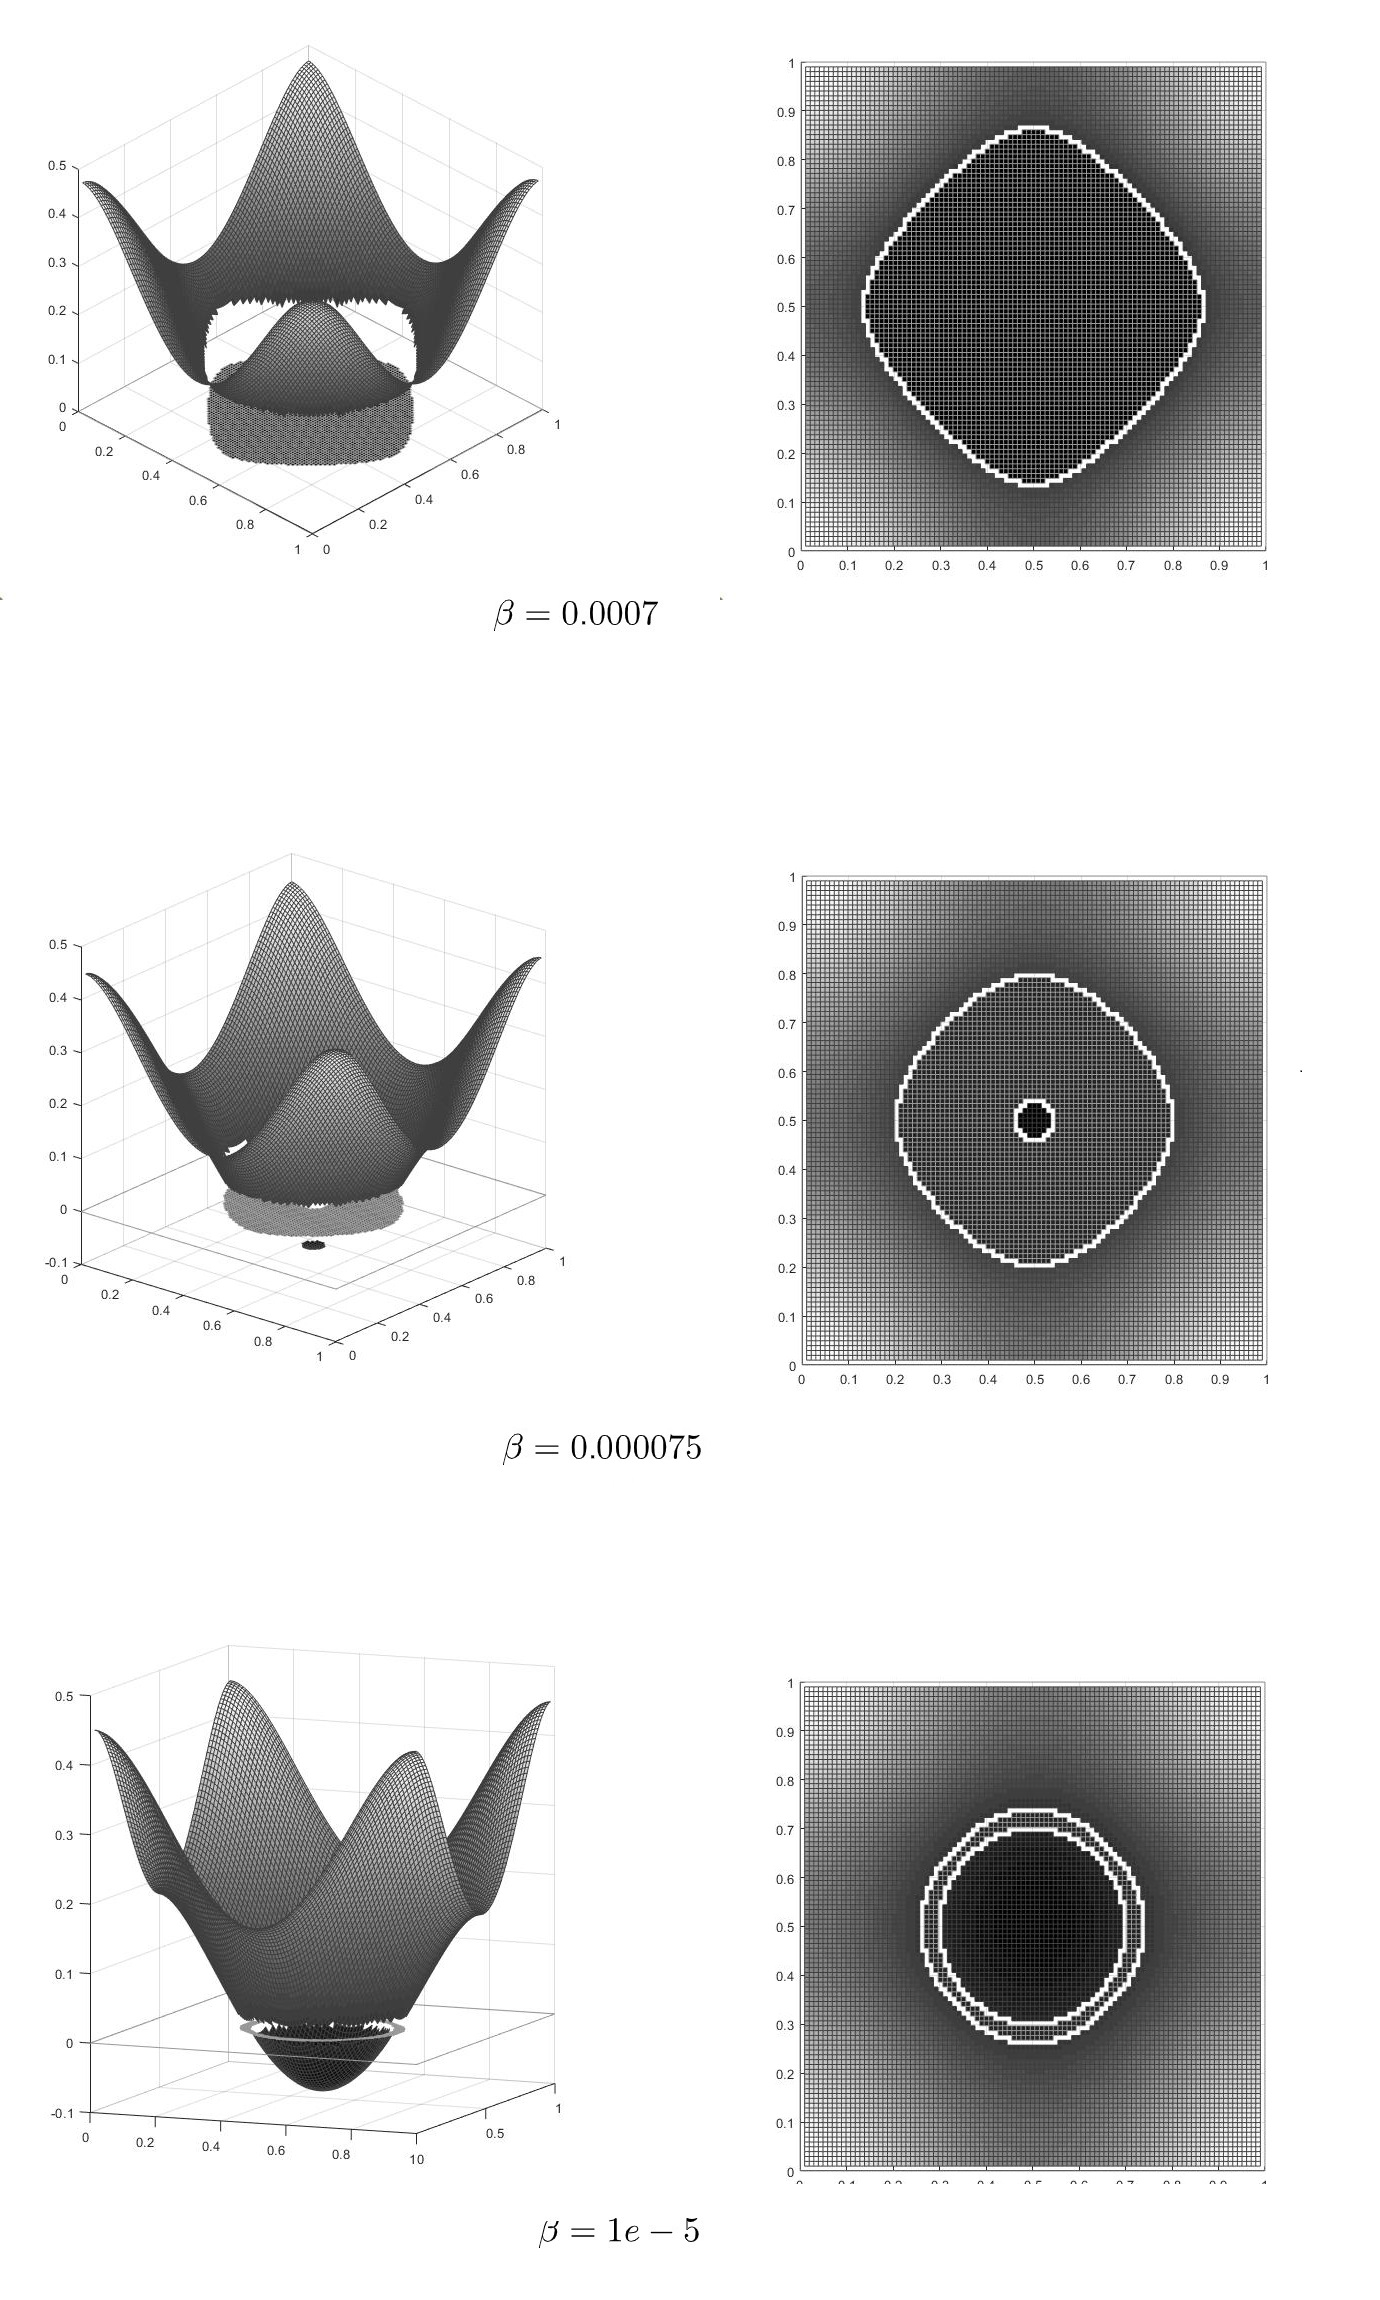
\includegraphics[scale=0.35]{matrizb.jpg}
    \caption{Graphics of the optimal control $u$ (first column) and their supports (second column) as $\beta$ varies. The first row correspond to the solution when $\beta=0.0007$, the second corresponds to $\beta=0.000075$ and third corresponds to $\beta=1e-5$. We notice that, as $\beta$ decrease, the support of function increase.}    
\end{figure}


\begin{figure}[H]
    \centering
    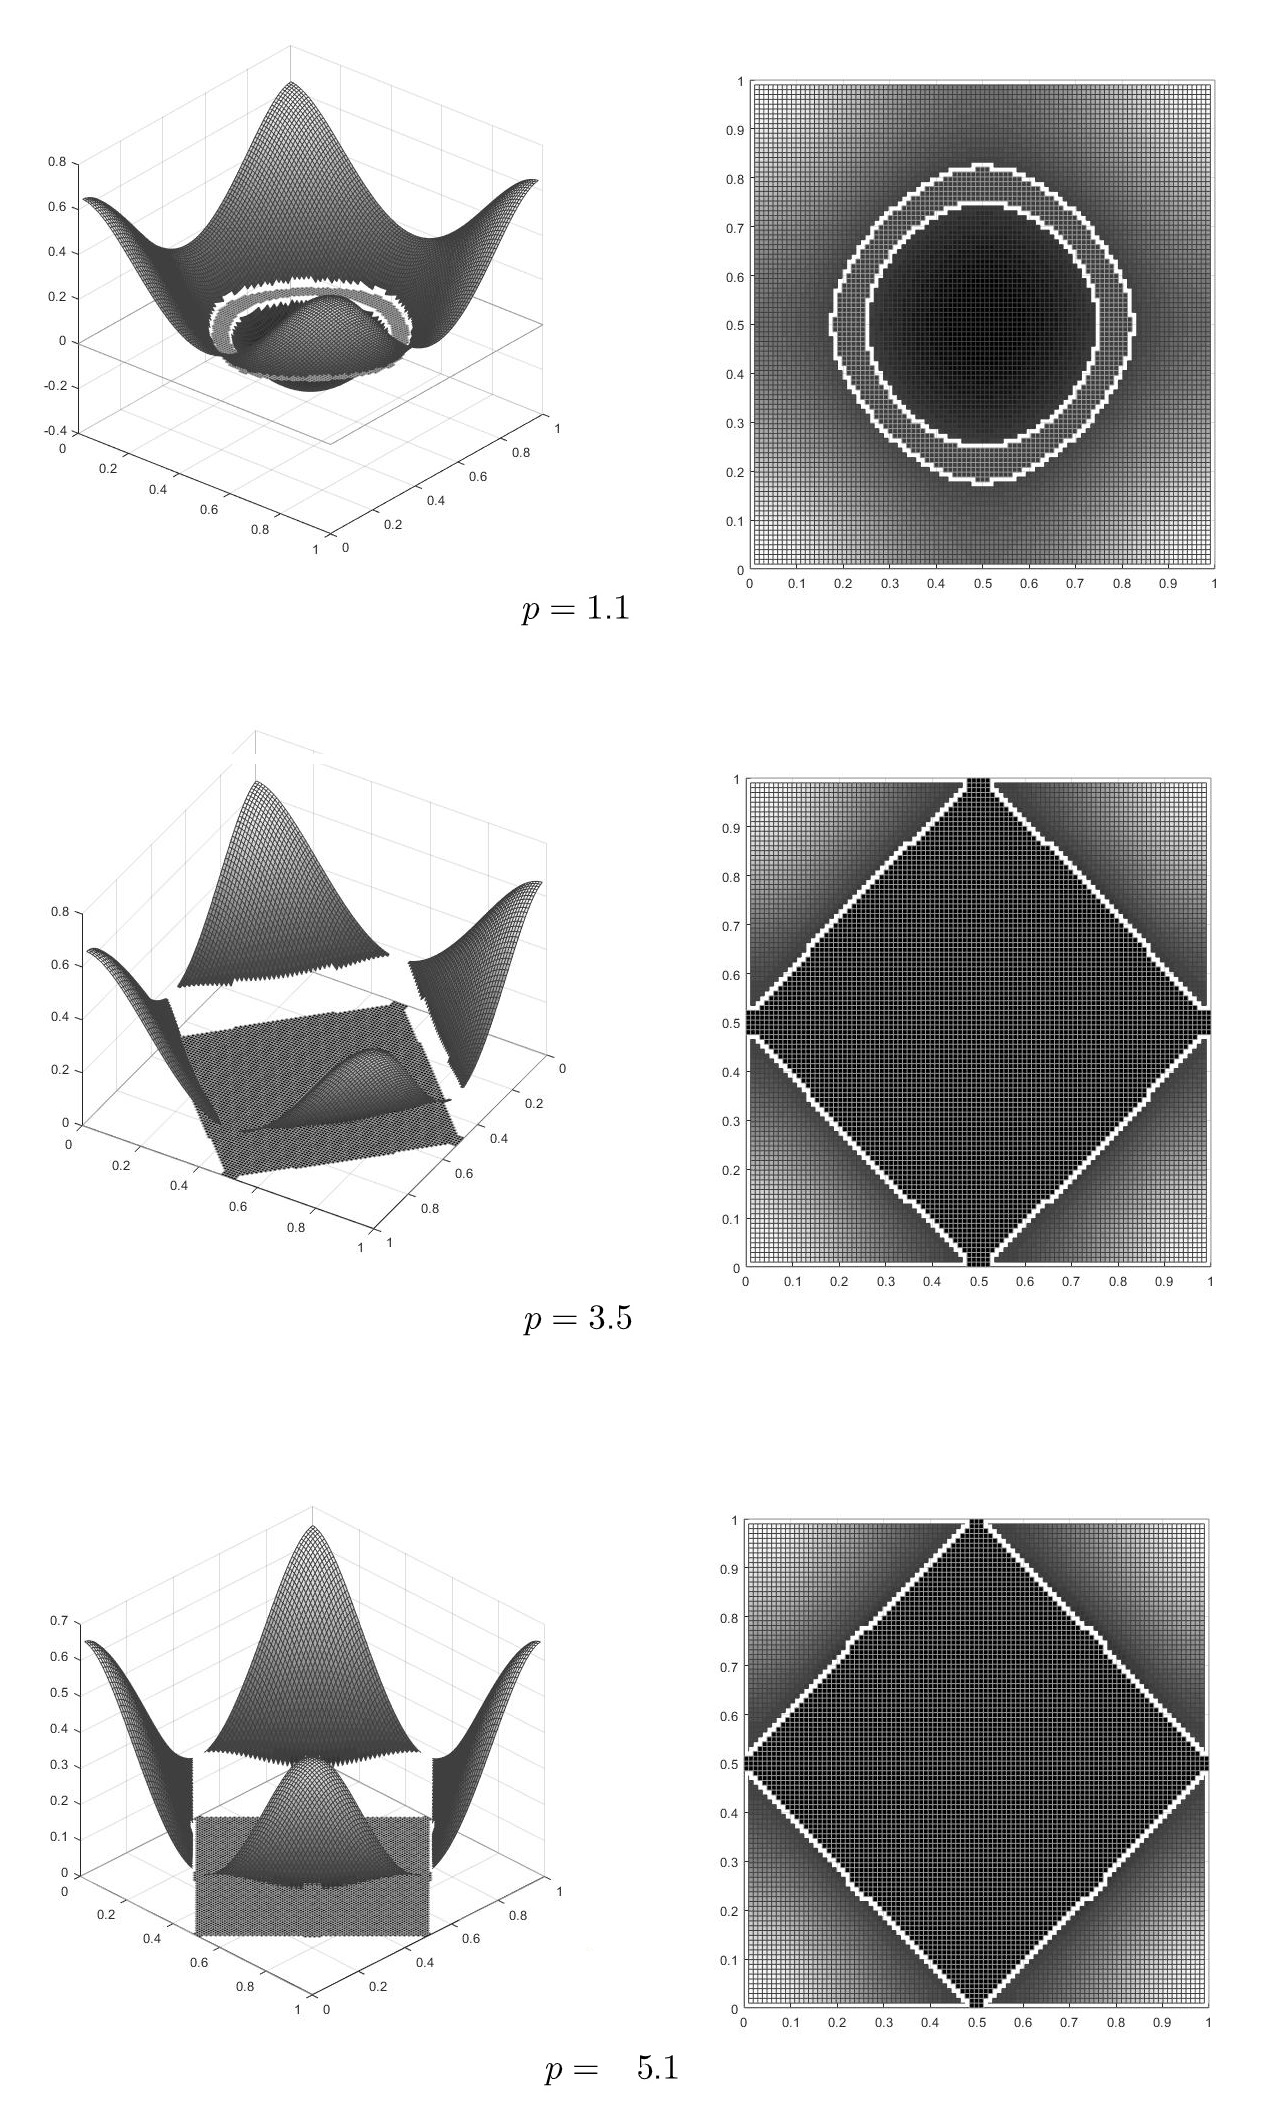
\includegraphics[scale=0.35]{matrizp.jpg}
    \caption{Graphics of the optimal control $u$ (first column) and their supports (second column) as $p$ varies. The first row correspond to the solution when $p=1.1$, the second corresponds to $p=3.5$ and third corresponds to $p=5.1$. We notice that, as $p$ increase, $q=\frac{1}{p}$ decrease and the support of function decrease, too.}   
\end{figure}

\newpage

We can see that the  optimal cost of the problem, such as  the null elements of $u$ tends to be constant. Even the number of iterations tends to be constant, too. The graphic of the optimal control and state for the higher value of $\gamma$ are presented in Figure 6.
\begin{figure}[h]
    \centering
    \begin{minipage}{0.5\textwidth}
        \centering
        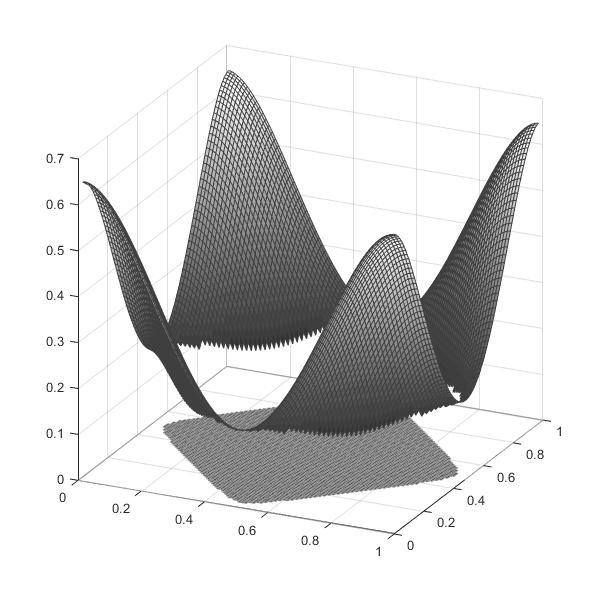
\includegraphics[width=0.7\textwidth]{ug.jpg} % first figure itself      
    \end{minipage}\hfill
    \begin{minipage}{0.5\textwidth}
        \centering
        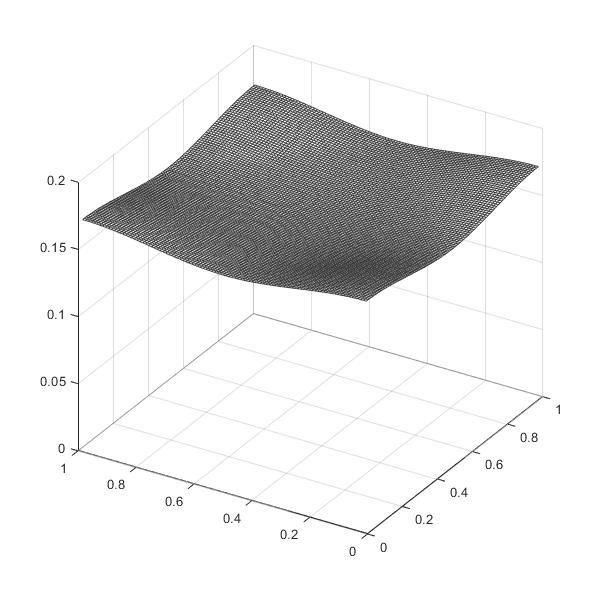
\includegraphics[width=0.7\textwidth]{yg.jpg} % second figure itself        
    \end{minipage}
    \caption{Optimal control (left) and state (right) for the limit problem when $\gamma=1e5$.}
\end{figure}



For the test of $\lambda$, we take $c_1=1000$ and $c_2=50$, $\alpha=1e-3, \beta=2e-5, p=2$. Numerical results are presented in Table 6.

\begin{table}[h]
    \centering
    \begin{tabular}{|c|c|c|c|c|}
    \hline
    $\lambda$ & Optimal cost & Null elements in $u$ & Number of iterations\\
    \hline
    1e-4&0.0049671&5544&38\\
    1e-5&0.004967&5528&62\\
    1e-6&0.004967&5528&62\\
    1e-7& 0.004967 &5528  & 62\\  
    \hline
    \end{tabular}
    \caption{Variations of $\lambda$}
\end{table}
 Again, we can see that as $\lambda$ tends to decrease, optimal cost and null elements in $u$ tends to be constant. Graphical solutions are shown in Figure 7 
\begin{figure}[h!]
    \centering
    \begin{minipage}{0.5\textwidth}
        \centering
        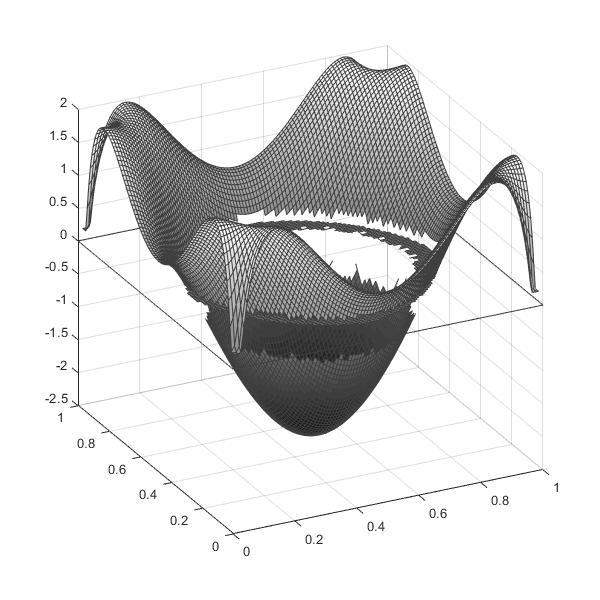
\includegraphics[width=0.7\textwidth]{ul.jpg} % first figure itself      
    \end{minipage}\hfill
    \begin{minipage}{0.5\textwidth}
        \centering
        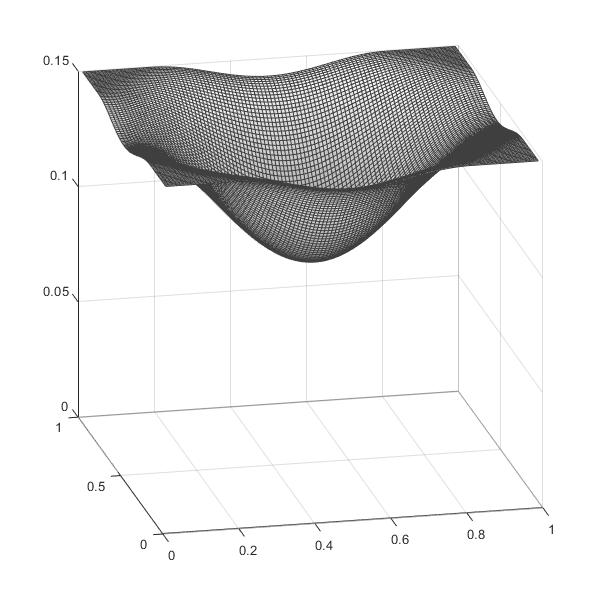
\includegraphics[width=0.7\textwidth]{yl.jpg} % second figure itself        
    \end{minipage}
    \caption{Optimal control (left) and state (right) for the limit problem when $\lambda=1e-7$.}
\end{figure}


\newpage
\newpage


The experiments presented before always report that $y$ is point wise strictly inside the bounds $y_a=-1$ and $y_b=0.2$, and therefore we can not see the real utility of Lavrentiev regularization in our problem; this motivate us to change the upper bound to $y_b=0.15$ and test again  our algorithm, varying $\lambda$ and reporting the number of point wise evaluations of $y$ which are significantly equal to $0.15$. Here, we take  $c_1=1000$ and $c_2=50$, $\alpha=1e-3, \beta=2e-5, p=2$. Table 7 report the variation of the active restrictions that are reached by $y$, as $\lambda$ tends to decrease
\begin{table}[h]
    \centering
    \begin{tabular}{|c|c|c|c|c|}
    \hline
    $\lambda$ & Optimal cost & Active restrictions in $y$ & Number of iterations\\
    \hline
    1e-3&0.0043199&0&28\\
    1e-4&0.0043155&848&43\\
    1e-5&0.0043182&896&62\\
    1e-6&0.0043187&906 &91\\  
    1e-7&0.0043185&904&67\\
    1e-8&0.0043185&904&67\\
    \hline
    \end{tabular}
\end{table}
We observe that as $\lambda$ tends to zero, the number of active restrictions of $y$ tends to increase until a stabilization of $904$. The optimal cost, however, tends to be constant. This show us that the state at the limit of $\lambda$ satisfies all the point wise  restrictions, even which equality. Now, the multiplier $\mu$ introduced in the optimal system associated to the semi smooth scheme developed in this section should satisfies the complementary conditions. Figures 8 and 9 show the optimal state and multiplier $\mu$ in the limit case $\lambda=1e-7$.
\begin{figure}[h]
    \centering
    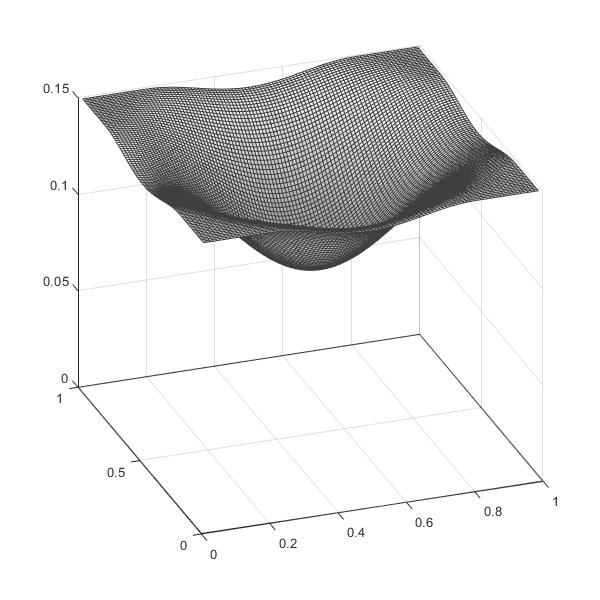
\includegraphics[scale=0.3]{yact.jpg}
    \caption{Optimal state in the limit case $\lambda=1e-7$}
\end{figure}

\newpage

\begin{figure}[H]
    \centering
    \begin{minipage}{0.5\textwidth}
        \centering
        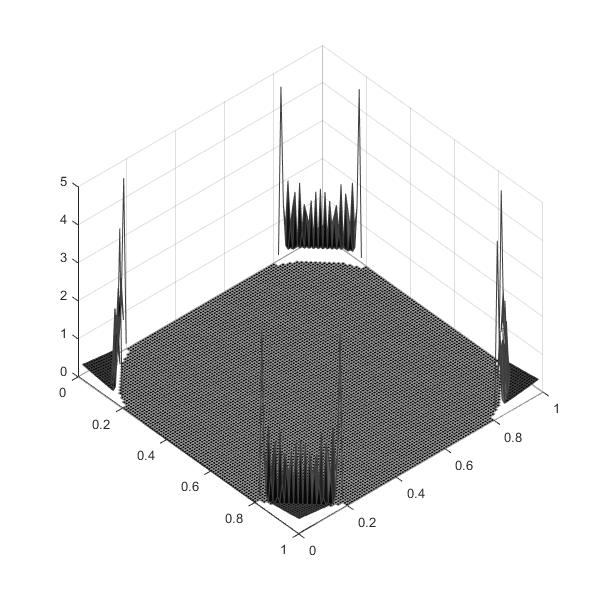
\includegraphics[width=0.8\textwidth]{mu.jpg} % first figure itself      
    \end{minipage}\hfill
    \begin{minipage}{0.5\textwidth}
        \centering
        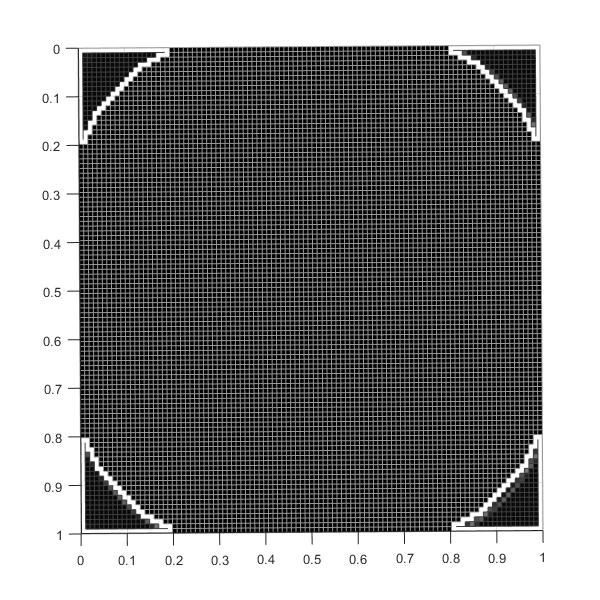
\includegraphics[width=0.8\textwidth]{musop.jpg} % second figure itself        
    \end{minipage}
    \caption{Graphic of the multiplier $\mu$ and its support}
\end{figure}

We can see that the support of $\mu$ coincides with the zones of $y$ which are strictly inside the interval $[-1,0.15]$. This implies that the complementary condition is satisfied in this region. On the other hand, when $y$ is active, $\mu$ takes other values than $zero$.

\section{Conclusions}
In this work we can prove the existence of solution for problem \eqref{P} using a Convex regularization of the problem, also called $\Gamma$ regularization. The point wise restrictions impossed to the state are carry out using a Lavrentiev regularization, which allow us to generate a family of convexified problems $(PC_{\lambda_n})_{n\in \mathbb{N}}$ which their solutions tend to a optimal solution for \eqref{P}.  For the numerical treatment of the problem, we developed a Semi-smooth Newton method with Lagrange multipliers in $L^2(\om)$, which ease the numerical treatment of the problem. This multipliers appear from the Lavrentiev regularization of \eqref{P}. The semi-smooth scheme has been developed from an optimal system arisen from the DC theory, using a Huber type regularization for the treatment of the nonconvexity of the problem.\\

Experimentally, we confirm that the quasinorm term present in \eqref{P} induces over $u$ sparsity in regions of the domain of the control that does not have necessary zero measure. This can be corroborated in the experiments when $\alpha$ and $\beta$ are varied separately. Is a interesting fact that the exponent of the quiasinorm $q=1/p$ influence over the sparsity of $u$ too.\\

Respect to the regularization parameters $\gamma$ and $\lambda$, we see that, through their variations tending to a limit ($\gamma\to \infty$ and $\lambda\to 0$) the numerical results tend to stabilize in an optimal solution; fact that we expected to have. In the case of the point wise restrictions of $y$, we see that $\mu$ satisfies the complementary conditions imposed in the optimal systems.\\

The globalization of the semi-smooth Newton method should be used for improving the numerical development of the algorithm. This fact is not used in the present investigation and might be considered in future researchs.






\begin{thebibliography}{99}

\bibitem{ambrosetti}
Ambrosetti, A.; Prodi, G., A Primer of Nonlinear Analysis. Cambridge, Cambridge University Press 1993. VIII, 171 pp., £ 25.00 H/b. ISBN 0-521-37390-5 (Cambridge Studies in Advanced Mathematics 34)

\bibitem{combettes}
Bauschke, H. H., and Combettes, P. L. Convex Analysis and Monotone Operator Theory in Hilbert Spaces, 2011. CMS books in mathematics).

\bibitem{bik}
Maïıtine Bergounioux, Kazufumi Ito and Karl Kunisch. “Primal-dual Strategy for Constrained Optimal Control Problems”. In: SIAM Journal on Control and Opti- mization 37, no 4 (1999), pp. 1176-1194.

\bibitem{bk}
Maïıtine Bergounioux and Karl Kunisch. “On the structure of Lagrange multipliers for state-constrained optimal control problems”. En: Systems Control Lett. 48 (mar. de
2003), pp. 169-176.

\bibitem{casas}
Eduardo Casas. Control of an Elliptic Problem with Pointwise State Constraints. In: SIAM Journal on Control and Optimization 24. (1986), pp. 1309-1318.

\bibitem{casasclason}
Eduardo Casas, Christian Clason, and Karl Kunisch. Parabolic control problems in measure spaces
with sparse solutions. SIAM Journal on Control and Optimization, 51(1):28-63, 2013.

\bibitem{casas-delosreyes}
Casas, Eduardo, Juan Carlos De Los Reyes, and Fredi Tröltzsch. "Sufficient second-order optimality conditions for semilinear control problems with pointwise state constraints." SIAM Journal on Optimization 19.2 (2008): 616-643.

\bibitem{casas-kunisch}
Casas, Eduardo, and Karl Kunisch. "Optimal control of semilinear parabolic equations with non-smooth pointwise-integral control constraints in time-space." Applied Mathematics \& Optimization 85.1 (2022): 12.

\bibitem{casaskruse}
Casas, Eduardo, Florian Kruse, and Karl Kunisch. "Optimal control of semilinear parabolic equations by BV-functions." SIAM Journal on Control and Optimization 55.3 (2017): 1752-1788.



\bibitem{delosreyes}
J.C De los Reyes. Theory of PDE-constrained optimization. Springer, Berlin, (2015).

\bibitem{dihn}
Pham Dinh, Tao and Le Thi and  Hoai An, Recent Advances in DC Programming and DCA,Springer Berlin Heidelberg, (2014), pp. 1-37.

\bibitem{donoho}
D.L.Donoho. ,Compressed sensing. IEEE Trans.Inform.Theory,52, 2006, pp. 1289-1306

\bibitem{eck}
I. Ekeland and R. Temam, Convex Analysis and Variational Problems, SIAM, Philadelphia, 1999.

\bibitem{hintkun}
M. Hintermüller and Karl Kunisch, Stationary optimal control problems with pointwise state constraints, SIAM Journal on Optimization, (2007). 

\bibitem{hinttv}
M. Hintermüller and T. Wu, Nonconvex TVq-Models in Image Restoration: Analysis and
a Trust-Region Regularization Based Superlinearly Convergent Solver, preprint, 2012.

\bibitem{ito-kunish}
K. Ito y K. Kunisch. Optimal control with $L^p(\om)$, $p \in [0,1)$, control cost. SIAM, J. Control optim. 2014 Society for Industrial y Applied Mathematics Vol.52,No.2,
2014, pp. 1251-1275.

\bibitem{kr}
Karl Kunisch and Arnd Rösch. “Primal-dual active set strategy for a general class
of constrained optimal control problems”. En: SIAM Journal on Optimization 13.2
(2002), pp. 321-334.

\bibitem{merino}
Pedro Merino. A difference-of-convex functions approach for sparse PDE optimal control problems with nonconvex costs. Comput Optim Appl 74. Springer Science+Business Media. (2019), pags. 225-258.

\bibitem{merino1}
Pedro Merino. A Semismooth Newton Method for Regularized Lq-quasinorm Sparse Optimal Control Problems. Numerical Mathematics and Advanced Applications ENUMATH 2019. Springer Nature Switzerland. (2019), pags. 723-731.

\bibitem{meyer1}
Chr. Meyer, U. Prüfert and F. Tröltzsch. “On two numerical methods for state-
constrained elliptic control problems”. In: Optimization Methods and Software 22.6
(2007), pp. 871-899.

\bibitem{mifflin}
R. Mifflin, Semismooth and semiconvex functions in constrained optimization, SIAM J. Control Optim., 15, (1977), pp. 959–972.

\bibitem{qi}
L. Qi, C-differential operators, C-differentiability and generalized Newton methods, Research Report
AMR96/5, School of Mathematics, University of New South Wales, Sydney, New South Wales, Australia (1996).


\bibitem{qisun}
L. Qi and J. Sun, A nonsmooth version of Newton’s method,
jMath. Programming, 58, (1993), pp 353-367

\bibitem{rock} 
Tyrrell R. Rockafellar, R., Convex analysis, Princeton Mathematical Series, (1970).

\bibitem{stadler}
Georg Stadler, Elliptic optimal control problems with L1-control cost and applications for the placement of control devices, Computational Optimization and Applications, Volume 44, (2009), pp. 159-181

\bibitem{trol}
  F. Tröltzsch and J. Sprekels. Optimal Control of Partial Differential Equations: Theory, Methods, and Applications,Graduate studies in mathematics,American Mathematical Society, (2010)


\bibitem{ulbrich}
Ulbrich, Michael. Semismooth Newton methods for variational inequalities and constrained optimization problems in function spaces. Society for Industrial and Applied Mathematics, 2011.

\bibitem{valkonen}
Christian Clason and Tuomo Valkonen, Introduction to Nonsmooth Analysis and Optimization. 	arXiv:2001.00216, 2023

\bibitem{vogel}
 Curtis Vogel, Computational Methods for Inverse Problems, Society for Industrial and Applied Mathematics, (2002)

\bibitem{vossen}
 Georg Vossen, and Maurer, H., On $L^1$‐minimization in optimal control and applications to robotics,Optimal Control Applications and Methods, Volume 27, (2006), pp. 301-321. 
\end{thebibliography}
\end{document}






